\documentclass[preprint,12pt]{article}

\usepackage{cite}
\usepackage{amsmath,amsthm,amssymb,amsfonts}
\usepackage{graphicx}
\usepackage{textcomp}
\usepackage{multirow}
\usepackage{hyperref}
\usepackage{booktabs}
\usepackage{algorithm}
\usepackage{algpseudocode}
\usepackage{tabularx}
\usepackage{subcaption}
\usepackage{lipsum} % For lipsum
\usepackage[dvipsnames]{xcolor} % Custom Colors
% \usepackage{natbib}
\newcommand{\cm}[1]{\textit{{\color{blue}#1}}}
\newtheorem{lemma}{Lemma}



\begin{document}

%%
%% The "title" command has an optional parameter,
%% allowing the author to define a "short title" to be used in page headers.
\title{A Tiny, Human-Interpretable, Client-Side, Classifier}

%%
%% The "author" command and its associated commands are used to define
%% the authors and their affiliations.
%% Of note is the shared affiliation of the first two authors, and the
%% "authornote" and "authornotemark" commands
%% used to denote shared contribution to the research.

\author{Charles Meyers, Aaron P. MacSween, Tommy L\"{o}fstedt, and~Erik Elmroth}

\maketitle


\begin{abstract}
The recent developments in machine learning have highlighted a conflict between online platforms and their users in terms of privacy. 
The importance of user privacy and the struggle for power over their data has been intensified as regulators and operators attempt to police the platforms.
As users have become increasingly aware of privacy issues, client-side data storage, management, and analysis have become a favoured approach to large-scale machine learning.
However, state-of-the-art machine learning methods require vast amounts of labelled user data, making them unsuitable for models that reside client-side and only have access to a single user's data.
State-of-the-art methods are also computationally expensive, which degrades the user experience on compute-limited hardware and also reduces battery life.
% Classical machine learning methods often require fewer samples to be effective, but may not provide the same performance as large-scale neural networks, for instance.
A recent alternative approach has proven remarkably successful in classification tasks across a wide variety of data--- using only a small number of samples. 
The idea is to use a compression-based distance measure (called normalized compression distance) to measure the distance between objects in classical distance-based machine learning methods.
In this work, we demonstrate that the normalized compression distance is a pseudo metric; develop it for the wider context of kernel methods to allow modelling of complex data; present techniques to improve the training time of models that use this metric; and demonstrate state-of-the-art accuracy using the proposed methodology.
We show that the normalised compression distance is as accurate as other metrics and kernel methods---without incurring additional computational costs.
The end results is a simple, classification model with an accuracy that competes with state-of-the-art models while using only a fraction of their power, data, and compute requirements---with training times measured in seconds instead of days or weeks.
\end{abstract}





\section{Introduction}

Despite their efficacy across many domains, modern machine learning (ML) methods often have large numbers of parameters, and thus also require large numbers of samples to train~\cite{desislavov2021compute}. 
This aggregation of vast amounts of data creates numerous privacy, safety, and security threats~\cite{chat_control}---especially in the context of large neural networks---that are consequences of large-scale user data collection by platform operators (see Section~\ref{threat} for more details).
We propose an alternative method that uses compression algorithms to measure the distance between samples and incorporate this distance in a kernel for classification. The proposed method requires a remarkably small number of samples.
% The proposed distance metrics and kernels do not require special hardware.
\cm{Additionally, when using small training sets, the models can be trained entirely on a client device without sharing private user data with the platform operator---allowing the model builder to circumvent many weaknesses associated with state-of-the-art methods~\cite{chat_control,power_consumption_ai}.}
We demonstrate the efficacy of the proposed approach in the context of malware detection, network intrusion detection, and spam detection and show that this approach is effective even when trained on a small number of samples.





\subsection{Threat Model}
\label{threat}

In the context of online platforms, data are collected from end-users using dubious amounts of consent~\cite{nouwens2020dark} and aggregated at massive scales~\cite{desislavov2021compute}. 
Such data collection on online platforms often creates privacy, safety, and security risks~\cite{chakraborty_adversarial_2018,meyers}. 
One such privacy risk is the periodic attempts by regulators to weaken encryption standards~\cite{amnesty_encryption} and create a permanent backdoor on every device in a given jurisdiction.
Platform operators also discuss with governments to scan client devices for illegal or offensive content~\cite{chat_control,apple_csam}, but existing proposals are no less risky to user privacy, safety, or security.
Privacy experts have denounced such approaches for numerous reasons: the ease of \textit{extracting} private training data~\cite{choquette2021label,fredrikson_model_2015,li2021membership} or the model~\cite{fredrikson_model_2015,orekondy2019knockoff,jagielski2020high,correia2018copycat,shokri2017membership} itself, the ability of a malicious user to induce false positives for other users when the model is trained on user data~\cite{rawat2022devil,shokri2020bypassing,gu2017badnets,saha2020hidden,aghakhani2021bullseye,turner2018clean,shafahi2018poison,geiping2020witches,souri2022sleeper} (\textit{poisoning} attacks), and the triviality of simply \textit{evading} the detection mechanism~\cite{carlini_towards_2017,dohmatob_generalized_2019,hopskipjump,biggio_evasion_2013,meyers,chakraborty_adversarial_2018,deepfool,hopskipjump}.

Current platform solutions often rely on large-scale ML methods that are trained on vast amounts of user data and federated across devices~\cite{apple_csam}---an approach that has been criticized by privacy experts~\cite{chat_control}. 
Examples of security risks include attacks against ML systems that target a model during training~\cite{biggio_poisoning_2013}, prediction~\cite{biggio_evasion_2013,deepfool,carlini_towards_2017}, and deployment~\cite{distributed_attacks,santos2021universal}. 
Even when access to a model by an adversary is limited, it is possible to induce a misclassification~\cite{hopskipjump}, reverse engineer the model~\cite{extraction_attack}, determine the model weights~\cite{jagielski2020high}, or infer the class-membership of new samples~\cite{bentley2020quantifying}. 
This raises profound questions for safety-critical systems~\cite{meyers} and legal questions about access and control of the underlying data~\cite{mitrou2018data,marks2023ai}.
Additionally, it has been shown that finding prototypical meta samples from the training set of large-scale ML models is trivial~\cite{chakraborty_adversarial_2018}. 
Even if the attacker only has access to a typical application programming interface (API), there are reliable ways to fool the model~\cite{hopskipjump}. 
In short, distributed and centralised training paradigms are both inherently fragile to malicious users and dangerous for user privacy, even if the resulting model lives on the user device (rather than in the cloud). 

Instead of relying on a model trained on massive amounts of user data, as is typical in large-scale ML applied to platform-level data, it is possible to categorically sidestep the aforementioned attacks with a model that runs entirely client-side which  reduces the attack surface to only adversaries that have access to data that users generally consider private (\textit{e.g.}, the contents of a message). 
That is, the attack surface is reduced and can be unique to each user, session, or device by using data from each user in isolation and training a model on that user's device. Client-side models would only need to share a single bit (the classification label in a binary classification context) with the platform operator---allowing those operators to serve user-specific contents without exfiltrating private data from their entire user base. 
However, not training a model on large amounts of collected user data means that such hypothetical client-side methods are at risk of not performing at the level of state-of-the-art large-scale methods.

Recently, Jiang \textit{et al.}~\cite{jiang2022less} proposed a remarkably successful approach: a parameter-free text classification method (denoted NCD-KNN) that exploits a compression-based distance measure, the \textit{normalized compression distance} (NCD)~\cite{ncd}, to classify objects using the k-nearest neighbours (KNN) method~\cite{shalev2014understanding}.




\subsection{Motivations}
The goal of the work was to explore the efficacy of NCD in the context of kernel classifiers and to produce a model  that can be trained on and used by each user in isolation from all others, categorically circumventing the privacy and security concerns associated with the collection and analysis of millions of user-generated data points. 
First, NCD has been demonstrated to be a \textit{universal} measure of similarity between two objects~\cite{ncd}--- where a value of 0 denotes absolute dissimilarity and a value of 1 denotes similarity.
Secondly, Jiang's analysis~\cite{jiang2022less} relies on many thousands of samples, which would be unsuitable for the proposed (client-side) implementation due to long run-times; their method also includes unnecessary, repeated calculations (see Section~\ref{pre_compute_compression}).
While other research examined topics like image classification~\cite{opitz2023gzip}, chemical classification~\cite{weinreich2023parameter}, and text classification~\cite{nishida2011tweet}, the ability of NCD to classify datasets that contain string, numeric, and categorical data (heterogenous datasets) remains unexplored.

Additionally, the original work~\cite{ncd} includes an error term that is subsequently ignored in recent research~\cite{opitz2023gzip,weinreich2023parameter,nishida2011tweet,jiang2022less}, which leads to problems outlined in Section~\ref{pseudometric}.
To the best of our knowledge, no research has addressed the problem of negative values for NCD as the original authors~\cite{ncd} insist that this measure is always positive. 
This is clearly demonstrated to be false in Section~\ref{pseudometric}.

% However, some pairs of strings yield NCD distances that do not follow the axioms listed in Section~\ref{metric_spaces} (see Figures~\ref{fig:synthetic_check} and~\ref{fig:real_world_check}).
% Section~\ref{pseudometric} details some string pairs that induce improper distances and Section~\ref{improvements} details the proposed mitigations and run-time improvements.
% This model normally uses NCD as a measure of distance~\cite{jiang2022less}.

Also, these prior works focused on distance-based ML methods (\textit{e.g.}, KNN), restricting the class of methods that can be considered and the kinds of data that can be analysed.
We extend the NCD to reproducing kernel Hilbert spaces and thus more elaborate ML methods---allowing for much more complex decision boundaries.

Furthermore, if run-time, storage, and computation requirements are minimised by building a model that is accurate on a small number of samples, then we can fulfil the goal of training a ML model entirely on a client device using data generated by a single user. 
In addition to a novel technique that uses NCD as a kernel, we propose several run-time improvements and modifications outlined in Sections~\ref{improvements}~and~\ref{modifications}.
% For example, that might mean marking an email as spam~\cite{ansuz_email} or examining the nearest neighbours of some text in a browser~\cite{ansuz_browser}.




\subsection{Contributions}
To use NCD, the model builder must choose a compression algorithm. 
While the effect of various compressors has been explored, in part, before~\cite{ncd_pitfalls}, but we expand the analysis in \cite{ncd_pitfalls} to newer compression algorithms and offer additional run-time improvements over the method of Jiang \textit{et al.} method.
The NCD-KNN method has shown very strong performance across several benchmarks, but Jiang \textit{et all's} implementation was not appropriate for real-time settings. 
However, NCD is a pseudo-metric~\cite{opitz2023gzip, weinreich2023parameter, nishida2011tweet, jiang2022less}, which means that applying ML methods blindly can lead to erroneous results (\textit{e.g.}, by incorrectly ordering the nearest neighbours).  
In this work we compile some examples of this non-metric behaviour Section~\ref{pseudometric} and propose techniques to mitigate the effects of this behaviour in Section~\ref{improvements}.
We also propose run-time improvements over the method of Jiang~\textit{et al.} (Section~\ref{improvements}).
Additionally, we expand the notion of NCD-as-a-distance~\cite{opitz2023gzip,weinreich2023parameter,nishida2011tweet,ncd,jiang2022less} to kernels (Section~\ref{kernels}) in an attempt to allow it to be used to model more complex decision boundaries than those allowed by distances alone.
That is, we propose NCD kernels; demonstrate how NCD is not a proper metric; offer run-time improvements over Jiang's method~\cite{jiang2022less}; 
and demonstrate the efficacy of the run-time optimised method on a variety of datasets. 
In this paper, we:

\begin{itemize}
    \item Demonstrate that normalized compression distance is not a metric (Section~\ref{pseudometric}) and propose techniques to make it behave more like a metric (Section~\ref{modifications}).
    % \item Discuss how private model deployment is safer by design (Section~\ref{threat}) and the efficacy of this design-constraint on several datasets (see Figure~\ref{fig:sample_size}).
    \item Develop a classifier (evaluated with KNN, logistic regression, and SVC) that offers large run-time improvements over other implementations discussed in the literature (Section~\ref{improvements}).
    % \item Provide efficient implementations of the proposed classifiers in \texttt{Java\-script} as well as a \texttt{Scikit-learn} compatible implementation in \texttt{Python}.
    \item Evaluate and empirically show the efficacy of the proposed compression-based classifiers across multiple binary classification datasets.
\end{itemize}



\section{Background}

In the sections below, we describe and define the NCD, summarize existing string metrics, define the distance matrix and how to calculate it, define some kernels and how to calculate the kernel matrix, and outline the method proposed by Jiang \textit{et al.}~\cite{jiang2022less}.



\subsection{Normalized Compression Distance}
\label{ncd}
The normalized compression distance (NCD; \cite{ncd}) is defined as
\begin{equation}
    \text{NCD}(x, x') = \frac{\mathcal{C}(xx') - \min\{\mathcal{C}(x), \mathcal{C}(x')\}}{\max\{\mathcal{C}(x), \mathcal{C}(x')\}} + \varepsilon,
\end{equation}
where $\mathcal{C}(z)$ is the length of the compressed form of the data, $z$, using a compression algorithm, $\mathcal{C}$, the notation $xx'$ denotes the concatenation of strings $x$ and $x'$, and $\varepsilon$ is an error accounting for imperfect compression algorithms~\cite{ncd}. This error is generally assumed to be small relative to the rest of the terms, but, as the original authors already noted, the resulting NCD values may be larger than one~\cite{ncd}.
Jiang \textit{et al.}~\cite{jiang2022less} proposed to use NCD in conjunction with the KNN classifier, but we extend this idea to other classifiers (\textit{e.g.}, SVCs~\cite{vapnik1994measuring}) that use measures of distance to cluster samples into classes. 
Since NCD requires the model builder to choose a compressor, we use the notation $\text{NCD}_{\text{gzip}}$ for \texttt{gzip}, $\text{NCD}_{\text{bz2}}$ for \texttt{bz2}, and $\text{NCD}_{\text{brotli}}$ for \texttt{brotli}. 
% section{NCD is a not a metric}
\label{pseudometric}
\label{metric_spaces}
While NCD is often discussed as a measure of distance~\cite{opitz2023gzip,weinreich2023parameter,nishida2011tweet,jiang2022less,ncd}, it does in fact not adhere to the axioms of metric spaces. 
Instead, as we will show here, it is a not a metric.

We denote the points $x_1,x_2,\ldots,x_n$  in a set $X$, and some distance function $d(x_1,x_2)$, where  $\mathbb{R}$ denotes the set of real numbers. 
A metric space is defined by some measure of distance ($d:X \times X \rightarrow \mathbb{R}$) between the constituent components of some space, usually called points. 
The distance function, $d$, and set of points,  $X$, are said to be a metric space if the following four axioms hold~\cite{metrics}:
\begin{align}
    d(x_1,x_2) &= 0 \iff x_1 = x_2 \qquad\text{(zero axiom)} \label{eq:axioms_zero}\\
    d(x_1,x_2) &\geq 0 \qquad\text{(non-negativity axiom)} \\
    d(x_1,x_2) &= d(x_2, x_1) \qquad\text{(symmetry axiom)} \\
    d(x_1,x_3) & \leq d(x_1,x_2) + d(x_2,x_3) \qquad\text{(triangle inequality axiom)} \label{eq:axiom_triangle_inequality}
\end{align}


Much of the literature devoted to NCD has treated it as a proper metric~\cite{opitz2023gzip,weinreich2023parameter,nishida2011tweet,jiang2022less}. However, it is not.
\begin{lemma}
    When using \texttt{gzip}, \texttt{bz2}, and \texttt{brotli} compressors, NCD does not adhere to the axioms in Equations~\ref{eq:axioms_zero}--\ref{eq:axiom_triangle_inequality}, and is thus not a metric.
\end{lemma}
\begin{proof}
    We show that NCD fails to adhere to the axiom for metrics by counter-examples in what follows.

    \vspace{0.5em}
    \noindent%
    \textit{Zero axiom:} The following counter-examples violate the zero axiom:
    $\text{NCD}_{\text{gzip}}(A,A) = .04$, $\text{NCD}_{\text{bz2}}(B,G) = 0 $, and $\text{NCD}_{\text{brotli}}(X,X) = .2$.

    \vspace{0.5em}
    \noindent%
    \textit{Non-negativity axiom:} The following counter-examples violate the zero axiom:
    $\text{NCD}_{\text{gzip}}(AAAA,AAAA) = -.04$, $\text{NCD}_{\text{bz2}}(AAAA,AAAA) = -.04$, and $\text{NCD}_{\text{brotli}}(AAAA,AAAA) = -.04$.
    \cm{TODO: Only gzip had negative values in my log file. Can try more combinations.}
    
    \vspace{0.5em}
    \noindent%
    \textit{Symmetry axiom:} The following counter-examples violate the zero axiom:
    $\text{NCD}_{\text{gzip}}(CCCCB, BCCA) = .2 \neq text{NCD}_{\text{gzip}}(BCCA, CCCCB)=.12$, $\text{NCD}_{\text{bz2}}(KC, CCC) = .11 \neq \text{NCD}_{\text{bz2}}(CCC, KC) = 0 $, and $\text{NCD}_{\text{brotli}}(CCAACCCCA, CBCA) = .62 \neq \text{NCD}_{\text{brotli}}(CBCA, CCAACCCCA) = .54$.

    \vspace{0.5em}
    \noindent%
    \textit{Triangle Inequality:} The following counter-examples violate the zero axiom. When $x= AAAAAAAAA, y=AAA, z=A$, $\text{NCD}_{\text{gzip}}(y,z) > \text{NCD}_{\text{gzip}}(x,y) + \text{NCD}_{\text{gzip}}(x,z)$. When $x= BC, y=AN, z=J$, $\text{NCD}_{\text{bz2}}(x,y) > \text{NCD}_{\text{bz2}}(x,z) + \text{NCD}_{\text{bz2}}(y,z)$. When $x= BCAC, y=CCBABCBAB, z=CCCCABCC$, $\text{NCD}_{\text{brotli}}(x,z) > \text{NCD}_{\text{brotli}}(y,z) + \text{NCD}_{\text{brotli}}(x,y)$
    
\end{proof}

% \subsection{Other Notation}

% Some additional notation is defined here. 
% We denote the cardinality of a set, $X$, as
% $$
%     | X |.
% $$
% For a matrix, $D$, $D_{ij}$ is the entry of $D$ in the $i$-th row and $j$-th column.
% 


\subsection{Calculating the distance matrix}
\label{distance_matrix}

Put the "Starting from Jiang ..." part here.

To use ML methods on string data, we need to find a set of numeric features that can be derived from a vector of samples.
To accomplish this, we calculate the pairwise distances between two sets of samples (denoted $X, X'$) to generate a \textit{distance matrix} ($D$) 
In addition, we propose modifications to this algorithm in Section~\ref{modifications}).
For the training step, $X = X'$ and, for prediction, it is assumed that $X \neq X'$.
While many of the above distance metrics are symmetric, this is, as we will see, not the case with NCD.
Algorithm~\ref{alg:vanilla} clearly shows that the run time associated with finding the distance matrix scales with $n = | X |, m = | X' |$, \textit{i.e.}, the run time is $\mathcal{O}(nm)$ for both compute and memory.
Clearly, if the number of samples in $X$ or $X'$ is large, then run-time becomes a major concern.
Additional modifications to calculating the pairwise distances between sets are outlined in Section~\ref{improvements}.






\subsection{Kernelisation}
\label{kernels}

% Whereas distance functions are used to measure the \textit{dissimilarity} between different examples, $x,x'$, a \textit{kernel-function}, $k$, is a measure of \textit{similarity} in an associated \textit{feature space}.
We propose to use NCD to construct an approximate kernel, allowing NCD to be used with a much larger set of ML methods than as a distance.

For our purposes, a kernel is defined as a symmetric function, $k : \mathcal{X} \times \mathcal{X} \rightarrow \mathbb{R}$, such that
\begin{equation}
    k(x, x') := \langle \phi(x), \phi(x') \rangle 
    \label{eq:kernel}
\end{equation}
for all $x, x' \in \mathcal{X}$,
where $\phi: \mathcal{X} \to \mathcal{Y}$ is a feature function (a function extracting features from its inputs), and $\langle \cdot, \cdot \rangle$ denotes an inner product in the feature space, $\mathcal{Y}$.
The $i$-th row and $j$-th column of a kernel matrix, $K$, is
$$
    K_{ij} = k(x_i, x_j).
$$
% Some kernels can be rewritten as a function of the distance between two points, such that.
% $$
%     K_{ij} = k(d(x_i,x_j))
% $$


If we are interested in Euclidean distances in the feature space, then we see that
\begin{align*}
    d(x,x')
        &= \| \phi(x) - \phi(x') \|_2^2 \\ 
        &= \langle\phi(x) - \phi(x'), \phi(x) - \phi(x') \rangle \\
        &= \langle \phi(x), \phi(x) \rangle + \langle \phi(x'), \phi(x') \rangle - 2\langle \phi(x), \phi(x') \rangle \\
        &= k(x, x) + k(x', x') - 2k(x, x').
\end{align*}
We denote this distance as the \textit{kernel distance}.

\label{rbf_kernel}

The radial basis function (RBF) kernel~\cite{kernels}, also known as the Gaussian kernel (when the distance is the Euclidean distance), maps an input space to an infinite-dimensional feature space, and is defined as
$$
    k(x, x') = \exp\left(-\frac{d(x, x')^2}{\lambda}\right),
$$
where $\lambda$ is a tunable parameter (denoted a \textit{length scale}) that controls how quickly the kernel function decreases as a function of the distance between points, \textit{i.e.}, determines the influence of individual points on neighbouring points.
The RBF kernel is particularly effective as it is known to be a universal function approximator~\cite{}.
% To use such a kernel with the outlined string distances, however, a pairwise distance matrix between all samples must be precomputed.
For the RBF kernel, when the symmetry and the zero axioms hold, we have that $k(x,x) = k(x',x') = 1$, and the kernel distance can be computed efficiently as
$$
    d_k(x, x') = 2 - 2 k(x, x').
$$



\section{Run-Time Improvements}
\cm{Move to methods section}
\label{improvements}
Starting from Jiang...



\subsection{Pre-computing the Compression vector}
\label{pre_compute_compression}

When computing the value of NCD$(x,x')$, it is necessary to calculate the values of $C(x)$ and $C(x')$. 
To classify a sample, Jiang \textit{et al.}~\cite{jiang2022less} iterated over the sets $X$ and $X'$ where $X$ is the set of samples with known labels and $X'$ has unknown labels. 
For $x_i \in X$ and $x_i' \in X'$, $C(x_i)$ and $C(x_i')$ are calculated repeatedly when calculating the pairwise distances between $X$ and $X'$.
Rather than do these unnecessary computations, our implementation compresses each entry in the $X$ and $X'$ once. 
Since compressing the input samples is the most costly part of this calculation, this saves significant run-time as shown in Section~\ref{results}.

\subsection{Symmetricisation}
\label{modifications}

We propose three new methods to induce adherence to the axioms listed above and compare their efficacy and run-time in Section~\ref{results}.
For the purposes of the experiments below, the method proposed by Jiang \textit{et al.}~\cite{jiang2022less} is denoted ``Vanilla'' and calculates the pairwise distance between two sets by finding every element of a distance matrix. 
The second method, which assumes symmetry by calculating the lower triangular matrix instead of the entire distance matrix, is denoted ``Assumed.''
Symmetry can be \textit{assumed} while calculating the distance matrix for a training set by using only the lower triangular portion of the distance matrix and then reflecting those values about the diagonal.
For some distance matrix, $D$, which rows and columns denoted by $i,j$ respectively, then the ``Assumed'' methodology calculates the lower triangular matrix in $D$ and then assumes that 
\begin{equation}
    D_{i,j} = D_{j,i}
    \label{eq:assumed}
\end{equation}
Secondly, symmetry can be \textit{enforced} by sorting the strings in the manner that is typical of several programming languages~\cite{}.
In contrast to the ``Assumed'' methodology that only modifies the training distance matrix, this method ensures that the symmetric behaviour occurs during prediction as well.
Thirdly, the \textit{average} value of $\text{NCD}(x,x')$ and $\text{NCD}(x',x)$ was used when calculating the distance matrix.
The average value of $\text{NCD}(x,x')$ and $\text{NCD}(x',x)$ is
$$
    \overline{\text{NCD}}(x,x') = \frac{\text{NCD}(x,x') + \text{NCD}(x', x)}{2}
$$
After simplifying and combining the error terms, this becomes
\begin{equation}
    \overline{\text{NCD}}(x, y) = \frac{\frac{\mathcal{C}(xx') + \mathcal{C}(x'x)}{2} - \min[\mathcal{C}(x), \mathcal{C}(x')]}{\max[\mathcal{C}(x), \mathcal{C}(x')]} + \varepsilon.
\end{equation}

\subsection{Zero-axiom check }
Additionally, to handle the case when $x_i = x_j$, we add a conditional statement and return a value of zero before any distances are calculated, as per the Zero axiom. 
We dub this process the ``Zero-axiom check''. 
The was conducted on the ``Assumed'' and ``Enforced'' methods, but not the ``Averaged'' method.


\subsection{Run Time Considerations}

While NCD is often treated as a metric, some implementations~\cite{jiang2022less} do not take advantage of the implied symmetry and calculate each pairwise entry of the distance matrix.
However, if symmetry is assumed, it can be used to reduce the run-time requirements by a factor of roughly 2 (for the ``Assumed'' and ``Enforced'' symmetry versions).
However, the run-time for the ``Averaged'' version is a little bit longer as the compressed string for the concatenation must be calculated twice---for $\text{NCD}(x,x')$ and $\text{NCD}(x',x)$ (see Section~\ref{eq:average}).
Because $\mathcal{C}(x), \mathcal{C}(x')$ are only computed once per sample (rather than repeatedly for each pairwise distance), the run-time of the ``Average'' method is approximately twice that of the ``Vanilla'' algorithm and four times that of the ``Assumed'' and ``Enforced'' variants with the advantage of being more theoretically sound.

% In this work, we propose two ways to improve the run-time of NCD when used as a distance measure for machine learning methods.
% First, we propose a rather trivial improvement to Jiang \textit{et al.}'s algorithm in Section~\ref{pre_compute_compression}.
% Second, we propose several modifications to the distance matrix computation algorithm outlined in Section~\ref{distance_matrix}, which are detailed below in Section~\ref{modifications}. 







\section{Experimental Methods}
\label{methods}

Several datasets, models, distance matrix computation algorithms (``Vanilla'', ``Assumed'', ``Enforced'' and ``Averaged''), and metrics ($\text{NCD}_{\text{gzip}}$, $\text{NCD}_{bz2}$, $\text{NCD}_{brotli}$, Levenshtein distance, Hamming distance, and Ratio distance) were used to evaluate the proposed methodology.
After generating the 5-fold cross validation sets for each dataset, the distance matrices for each distance matrix algorithm and metric were calculated, as outlined in Sections~\ref{distance_matrix}~and~\ref{modifications}.
Additionally, kernel matrices were found according to Section~\ref{kernels}.
Then, these distance and kernel matrices were provided to typical \texttt{scikit-learn} classifiers---KNN, logistic regression, and SVC.
To find the most appropriate hyper-parameters, each of the combinations enumerated above were evaluated using 5-fold cross validation. 
Then, to examine the trade-offs between accuracy and run-time, the number of training samples was varied on the set of hyper-parameters that was most consistently accurate during cross-validation for each dataset, model, distance matrix algorithm, and metric.
Process time was recorded for the distance matrix computation, as well as the model training and prediction times.
In addition, accuracy was recorded for all experiments.

To compare the effect of the distance matrix algorithms on the propensity to follow the axioms listed in Section~\ref{metric_spaces},

100 thousand string triplets were generated from the standard English alphabet (upper and lowercase) and exhaustively checked for adherence to the axioms.
Also, the training distance matrices found during cross-validation were evaluated for adherence to the axioms.



\subsection{Data}
\label{datasets}

Several open datasets were used to evaluate the efficacy of NCD in the context of heterogeneous tabular and text data.
We limit ourselves to strings here because some of the datasets are string data and the others are formatted as such for the experiments to allow for direct comparisons across all of the datasets.
We used KDD-NSL which is a log of system process data for both regular users (denoted benign) and malicious software (denoted adversarial)~\cite{kddnsl} which includes 6072 samples and 41 features that encapsulate the behaviour of both benign software and malware.
KDD-NSL includes software protocol, system error rate, whether the process has root privileges, and the number of files accessed by the process.
We also used the DDoS IoT dataset~\cite{ddos}, which includes information collected from network packet headers of adversarial and benign users across many types of DDoS attacks.
Specific features include source IP address, source port, destination IP address, destination port, and network protocol among a total of 90 features across more than 40 million samples, collected from both benign users and malicious traffic.
% To prepare the DDoS IoT dataset, the timestamp data was removed since the malicious and benign data were collected at different times and necessarily encodes the class label.
We used the Truthseeker dataset~\cite{truthseeker}, which includes 134 thousand messages from Twitter users with a label, provided by the data distributors, whether or not a given user was a suspected bot.
% While this dataset is normally includes metadata-- in an effort to examine the efficacy of NCD on text alone-- this work only included the ``tweet" and the ``BotScoreBinary'' label provided by the researchers who distribute the data (the classes represent regular users and suspected bot users).
Finally, we used the SMS Spam dataset~\cite{sms_spam} which includes SMS messages and a label indicating whether or not it is spam across 5575 samples.

In order to address class imbalances and ensure robust model evaluation, various sampling techniques were applied to the datasets. 
For several of the datasets, malicious examples were rare compared to the number of benign examples; therefore, each dataset was under-sampled~\cite{undersampling} using the \texttt{imblearn} package~\cite{imblearn} to ensure that the classes were balanced in each dataset. 
For each dataset, model, distance matrix algorithm, and distance metric, 1000 samples from each dataset were used to conduct five-fold cross validation, yielding five disjoint test sets of 200 samples each. 
Accuracy, distance matrix calculation time, and model training times, and prediction times were recorded for each of the 5 cross-validated folds.
After fitting each model for each dataset, distance matrix algorithm, measure of distance, and model-dependent hyper-parameters, the best-fit models were repeatedly trained on $m \in \{ 10, 20, 35, 60, 100, 200, 500, 1000\}$ samples and evaluated against 200 samples that were withheld during cross-validation with.



\subsection{Models}
\label{models}
NCD was evaluated both as a distance metric and as a kernel with several machine learning models and compared to standard string distances.
The distance matrices were calculated for each dataset, data fold, distance matrix algorithm (see Sections~\ref{distance_matrix} and~\ref{modifications}), and metric before being passed to a \texttt{scikit-learn} classifier---KNN, logistic regression, and SVC.
For each classifier, several hyper-parameters were evaluated using 5-fold cross-validation on the kernel matrices (see Section~\ref{kernels}).

K-Nearest Neighbors (KNN) uses the pairwise distances between labelled and new samples (distance matrix) to find the $k$-closest labelled samples.
In our experiments, $k 
\in \{1,3,5,7,11\}$, as odd numbers make ties impossible for binary classifiers.

Logistic regression is a statistical model used for binary classification where the probability of a sample belonging to a particular class is modelled as a linear combination of input features, transformed by a sigmoid function and a kernelised version exists~\cite{maalouf2011robust}.
In the presented experiments, an $\ell_2$ penalty term was tested as well as a configuration without any penalty. 
The coefficient of the penalty was in powers of 10 in the range $(10^{-3}, 10^3)$.
The \texttt{SAGA} solver~\cite{saga} was used with a tolerance of $10^{-4}$.

Support vector classifiers (SVCs) were used to classifier our datasets into one of two classes.
% The \texttt{scikit-learn} SVC implementation was used with the ``precomputed'' kernel option.
SVCs require a choice of value for a penalty term and we tested the range $(10^{-3}, 10^3)$ for each power of ten.










\subsection{Compressors}
\label{compressors}

To use NCD as a measure of distance, one must choose a compression algorithm.
We evaluated the \texttt{gzip}~\cite{gzip}, \texttt{bz2}~\cite{bz2}, and \texttt{brotli}~\cite{brotli_package} algorithms using their Pytho
For these experiments, we used the \texttt{gzip} and \texttt{bz2} modules that are part of the \texttt{Python} standard library, with default parameters.
For \texttt{brotli}, we used the \texttt{Python} package authored by Google~\cite{brotli_package}, also with default parameters.
Compared to \texttt{gzip}, the \texttt{bz2} algorithm is faster and decompression is slower due to the better compression ratio~\cite{bz2_comparison}, however those differences are negligible for the datasets used here (see Figure~\ref{fig:distance_time}) as the datasets we tested are much smaller than the documents, software, images, source code, audio, and operating systems tested in prior work~\cite{bz2_comparison}.

\subsection{Other measures of string distance}
\label{string_metrics}
To model datasets that comprise strings, several existing measures of distance between strings are routinely used~\cite{levenshtein}.
To evaluate the relative performance of the NCD metric, we compared it to several other common measures of string similarity, briefly outlined below.
% String Distances
\begin{itemize}
    \item \textit{Levenshtein:} is the ``edit distance'' or minimum number of single-character edits to transform one string into another~\cite{navarro2001guided}.
    \item \textit{Lev Ratio:} is the Levenshtein distance divided by the total length of the strings~\cite{levenshtein}.
    \item \textit{Hamming:} is the number of character positions where two strings differ. 
    \item \textit{Ham Ratio: is the number of character positions where two strings differ, divided by the length of the longer string.}
\end{itemize}





\section{Results and Discussion}
\label{results}

In this section, the results from the aforementioned experiments are discussed. 


\begin{figure}[p]
    \centering
    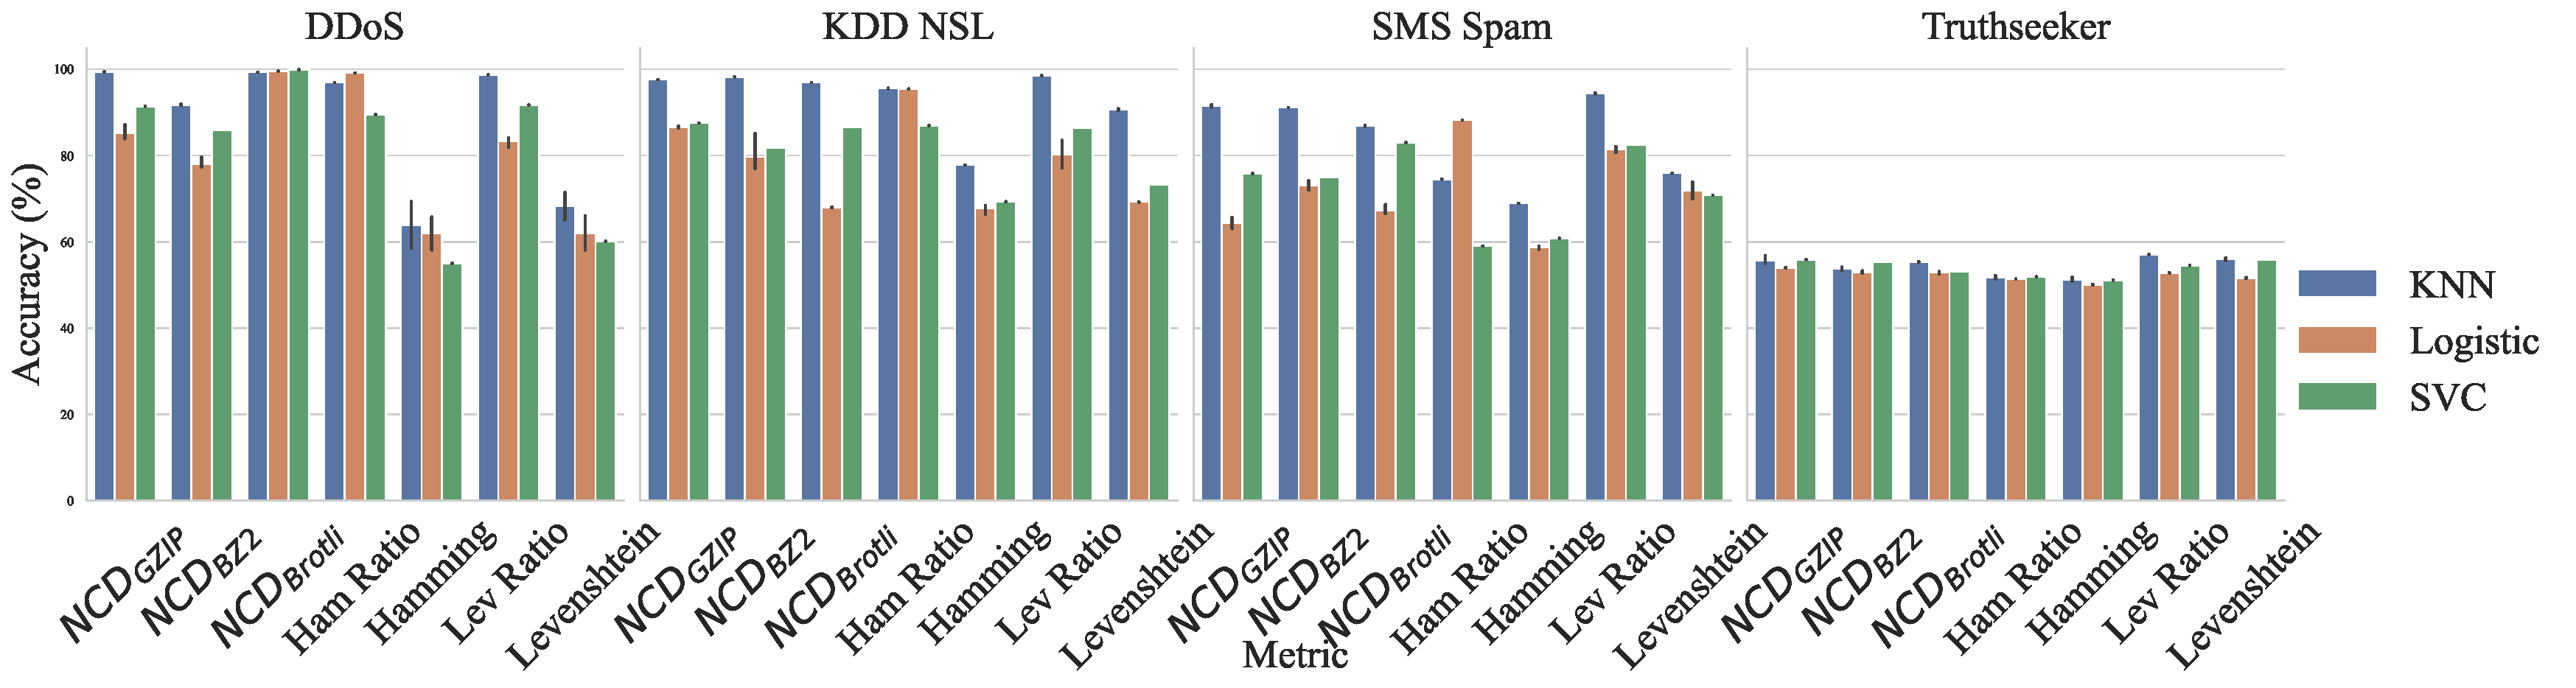
\includegraphics[width=0.99\textwidth]{images/accuracy_vs_metric.pdf}
    \caption{The accuracy across each dataset (columns), model (first-axis), and ML method (colour) for several different string metrics (first axis), calculated by averaging the scores of each fold in five-fold cross validation for each set of tested parameters (enumerated in Section~\ref{models}).}
    \label{fig:metric_acc}
\end{figure}



\subsection{Comparison of Different String Metrics}

Figure~\ref{fig:metric_acc} shows the classifier performance across each dataset and various string metric (and for NCD, with various compressors).
Across all datasets, the median and peak accuracy of the compressor-based metrics exceeds all the string metrics.

Figure~\ref{fig:distance_time} illustrates the run-times for the distance calculation time per sample, Figure~\ref{fig:train_time} illustrates the run-times for the model training time per sample, and Figure~\ref{fig:pred_time} illustrates the run-times for model prediction per sample.
NCD using various compressors is comparable in run-time to all other tested string metrics.
It is clear that run-times are largely comparable between NCD and the other string metrics for distance calculation time, training time, and prediction time.
% Please note that the training step is only necessary for certain configurations of the KNN method (\textit{e.g.}, when ball-tree or $k$-dimensional tree~\cite{knn_extensions} algorithms to learn features of the training set) and that the brute force version proposed by Jiang \textit{et al.}~\cite{jiang2022less} can skip this step entirely.
Overall, NCD (with GZIP, BZ2, and Brotli) offers comparable performance to the tested string metrics in terms of run-time. 

\subsection{Effect of Symmetricisation}

This work proposes several methods of symmetricisation for the distance matrix (Section~\ref{modifications}) and the efficacy of this modifications are examined below. 

\begin{figure}[p]
    \centering
    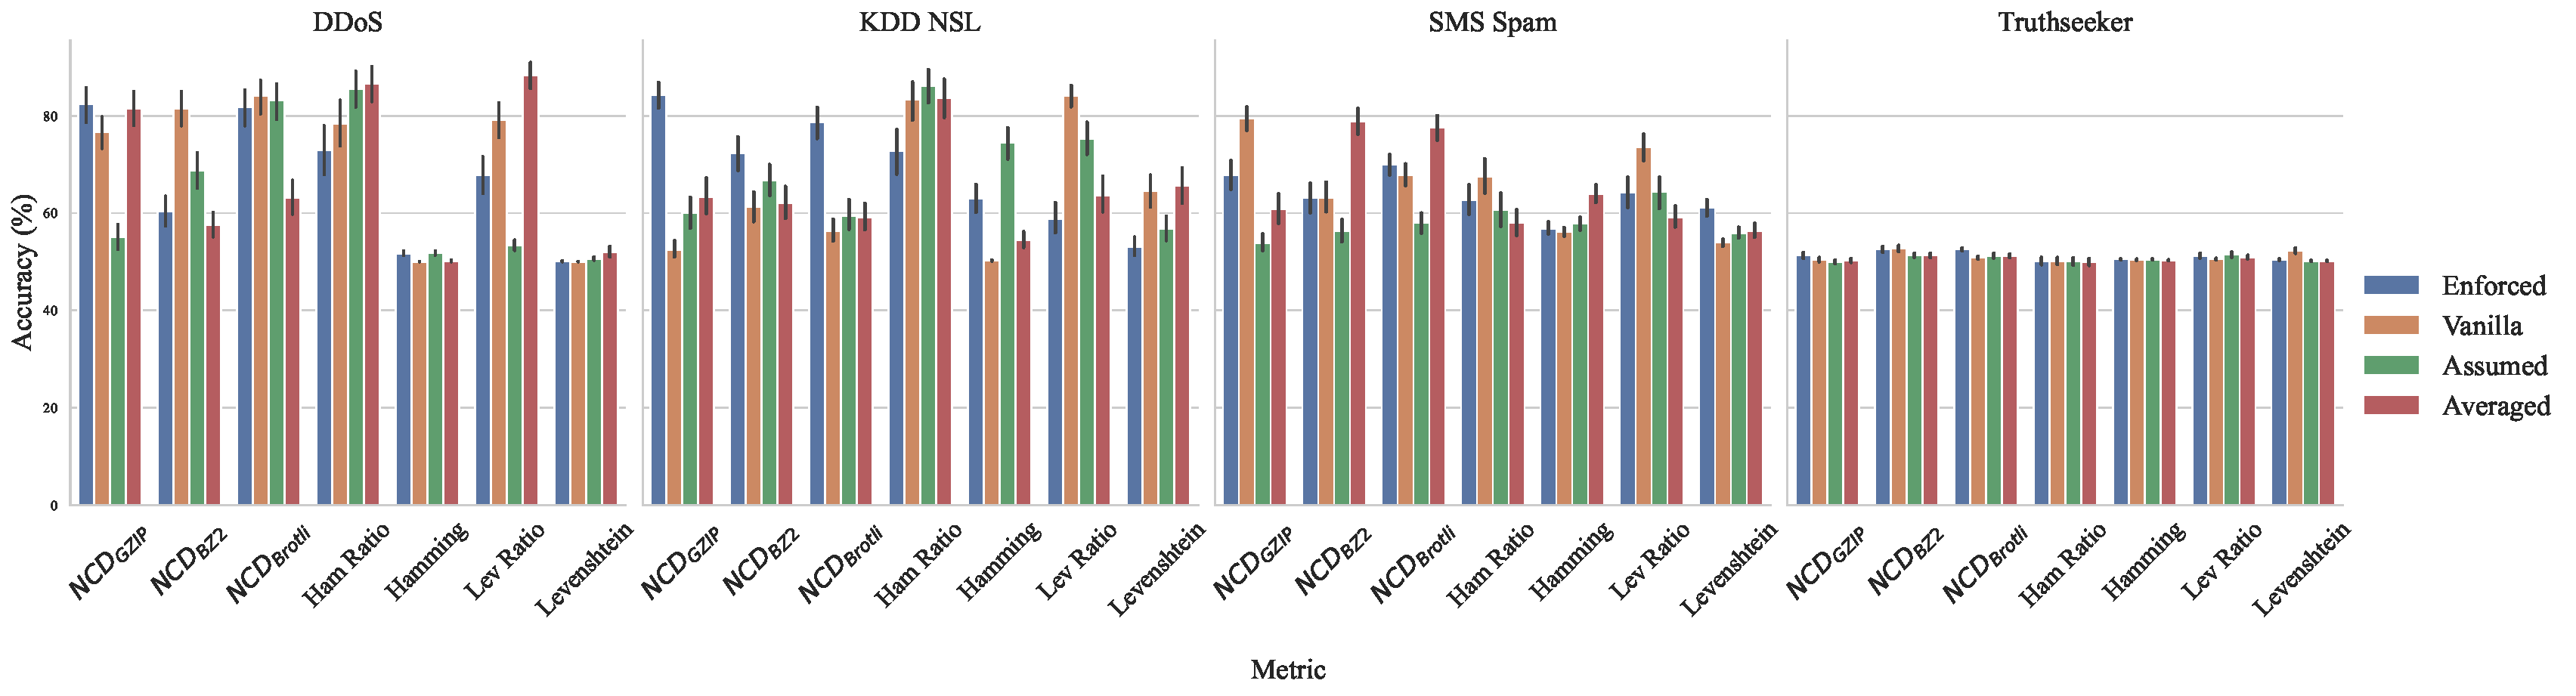
\includegraphics[width=0.99\textwidth]{images/accuracy_vs_symmetry.pdf}
    \caption{The accuracy across each dataset (columns),  and distance matrix computation algorithm (colour) for several different string metrics (first axis), calculated by averaging the scores of each fold in five-fold cross validation for each set of tested parameters (enumerated in Section~\ref{models}).}
    \label{fig:symmetric_acc}
\end{figure}
Figure~\ref{fig:symmetric_acc} shows the classifier performance across each dataset and various string metric (and for NCD, with various compressors).
There tends to be a significant difference in accuracy, depending on the dataset, symmetricisation algorithm, and metric. 
Figures~\ref{fig:synthetic_check}-\ref{fig:real_world_check} examine how the symmetricisation algorithms influence to what degree a given metric adheres to the axioms discussed in Section~\ref{metric_spaces}.  
Figure~\ref{fig:synthetic_check}...
Figure~\ref{fig:real_world_check}...
It is clear that \cm{TODO:}
\begin{figure}[h!]
    \centering
    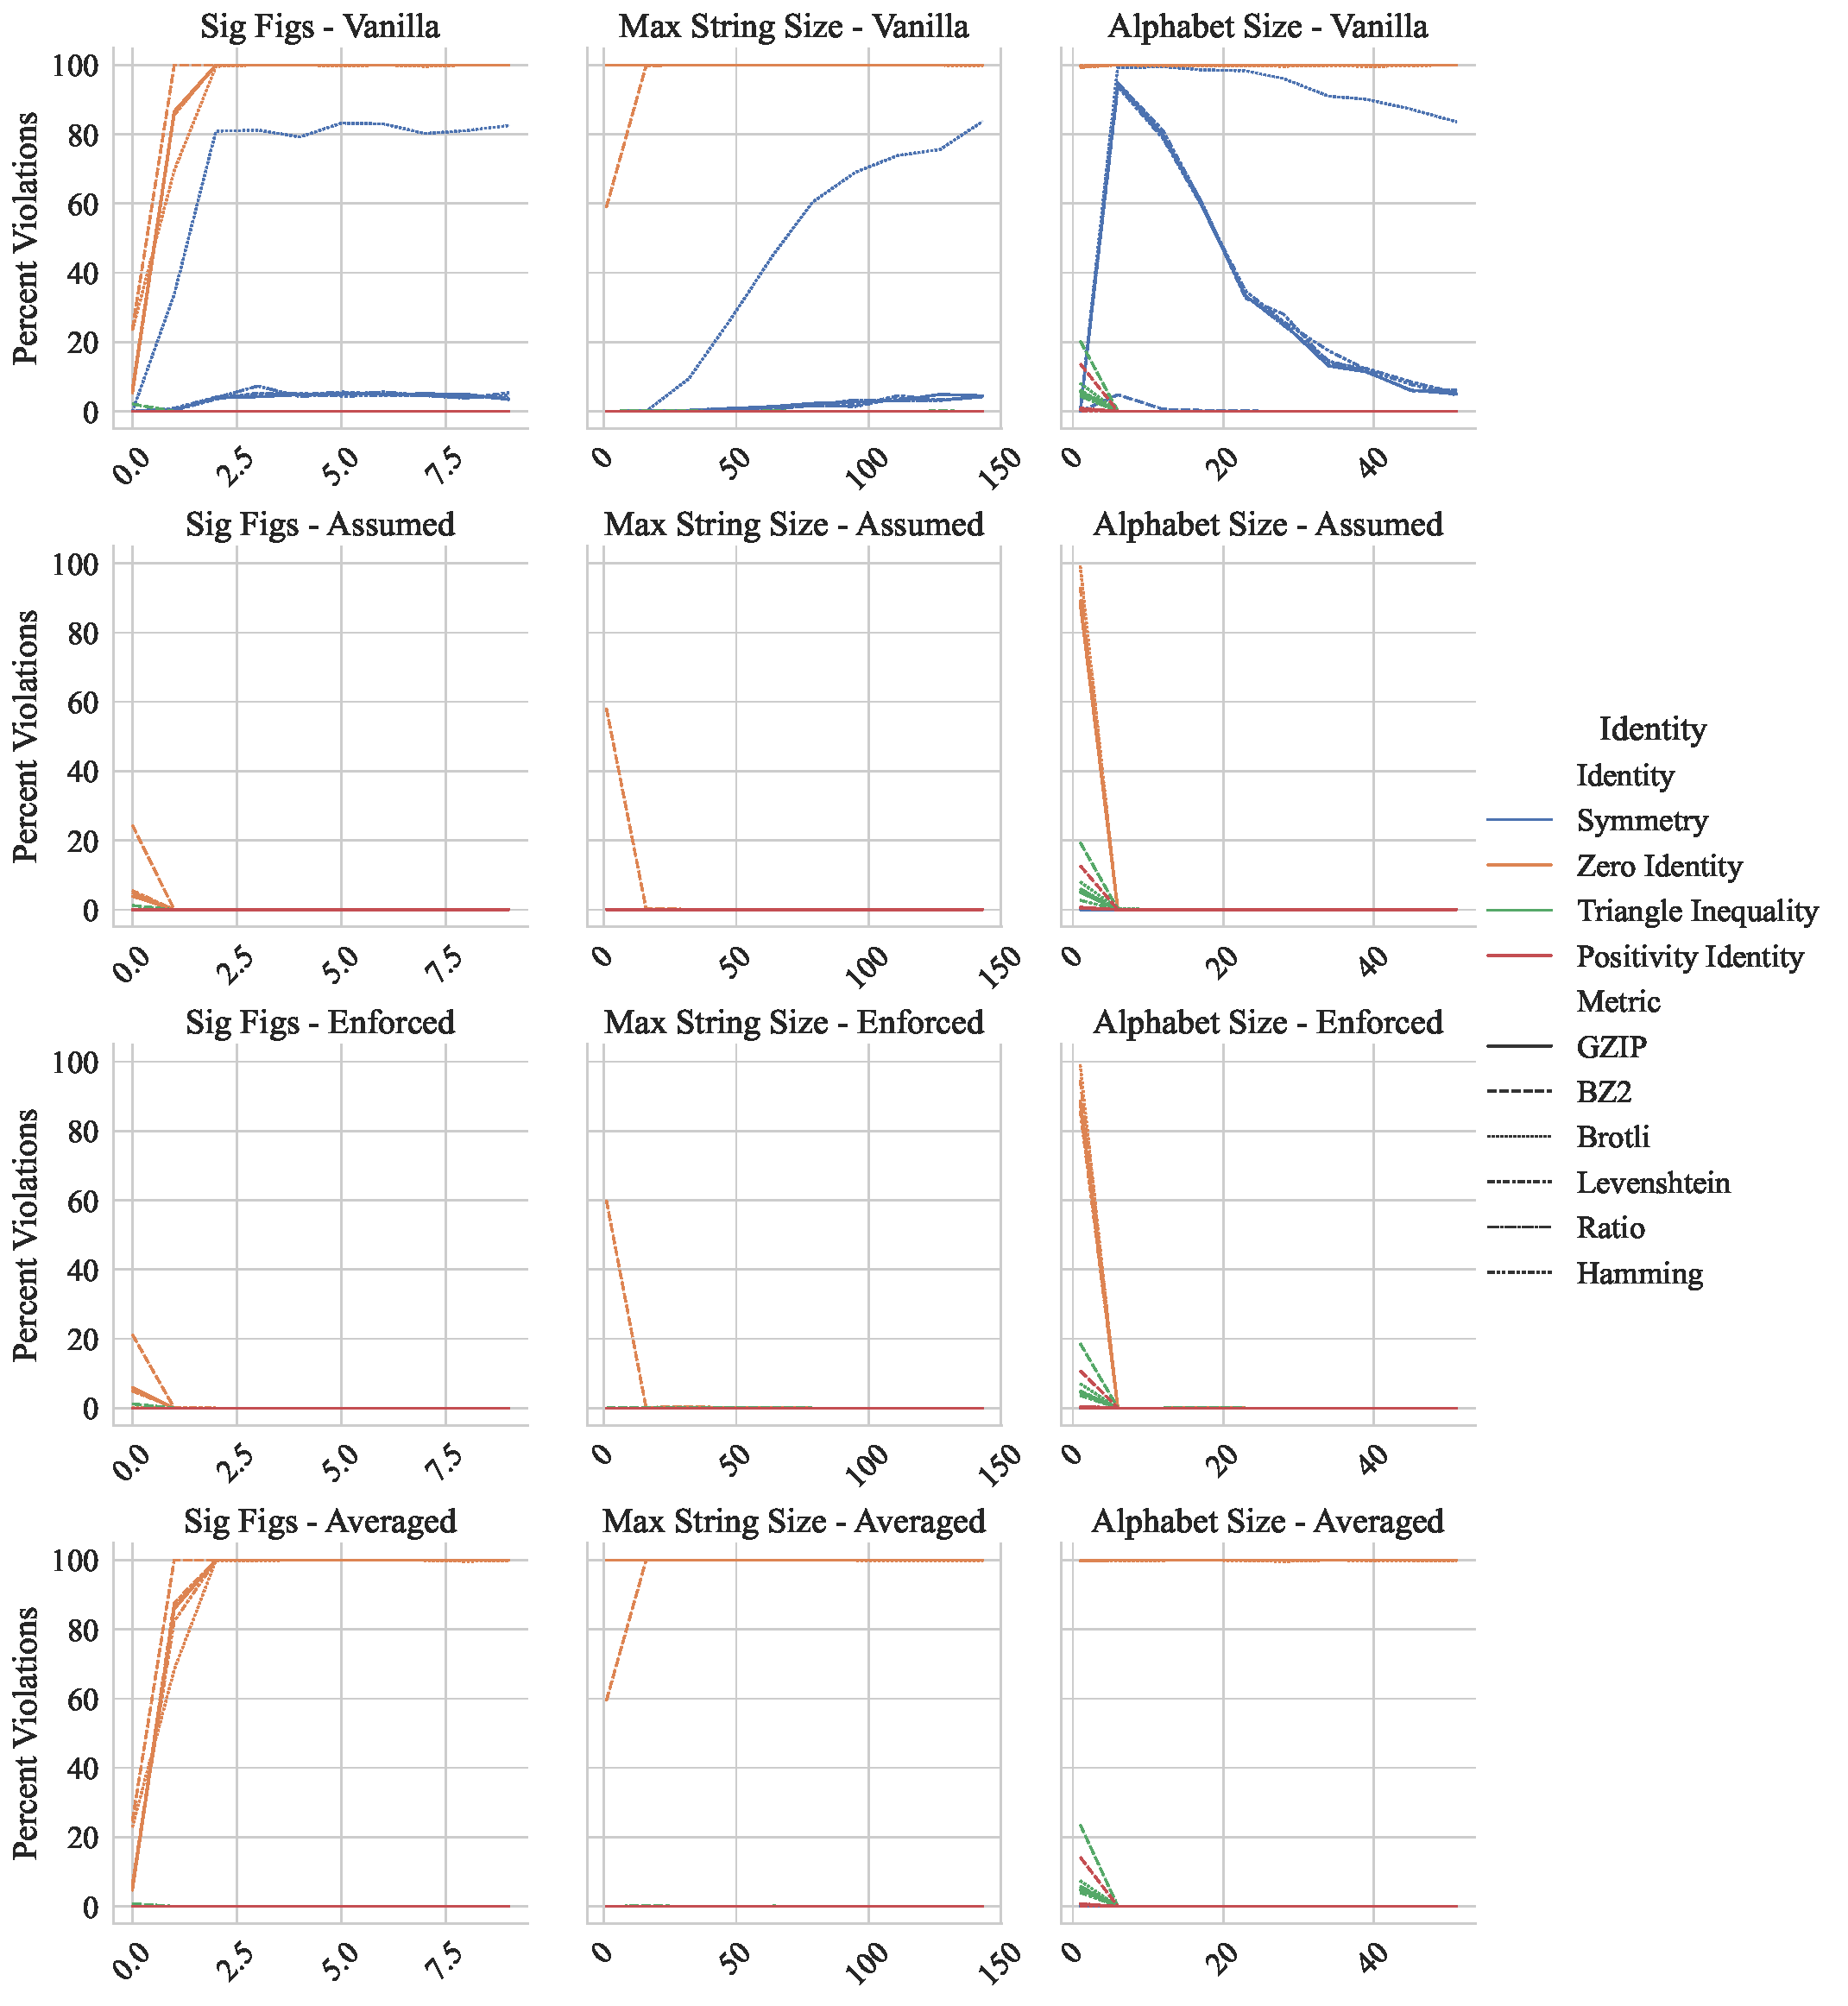
\includegraphics[width=0.70\textwidth]{images/synthetic_check.pdf}
    \caption{
    Percentage of examples found that violate the assumptions outlined in Section~\ref{metric_spaces} using the vanilla symmetricisation algorithm (top row), assumed symmetry (second row), enforced symmetry (third row), and averaged (Equation~\ref{eq:average}) algorithms on 100 thousand random strings generated from the standard English alphabet (upper and lowercase). 
    \textit{Sig Figs} refers to the number of significant figures. \textit{Max String Size} and \textit{Max Alphabet Size} refer to the number of characters and the number of unique characters respectively. 
    Unless otherwise specified by the x-axis in an individual plot, \textit{Max String Size}, \textit{Max Alphabet Size}, and \textit{Sig Figs} were all 144 characters (the character limit of a ``tweet''), 52 letters (upper and lower case English letters), and 10 significant digits. Each colour corresponds to a different axiom as defined in Section~\ref{metric_spaces} and each line marker corresponds to a different string distance as outlined in Section~\ref{compressors} and Section~\ref{string_metrics}. \cm{Here it says positivity instead of non-negativity, but that has been fixed locally and will be re-rendered when the ongoing experiments finish.}
    }
    \label{fig:synthetic_check}
\end{figure}

\begin{figure}[h!]
    \centering
    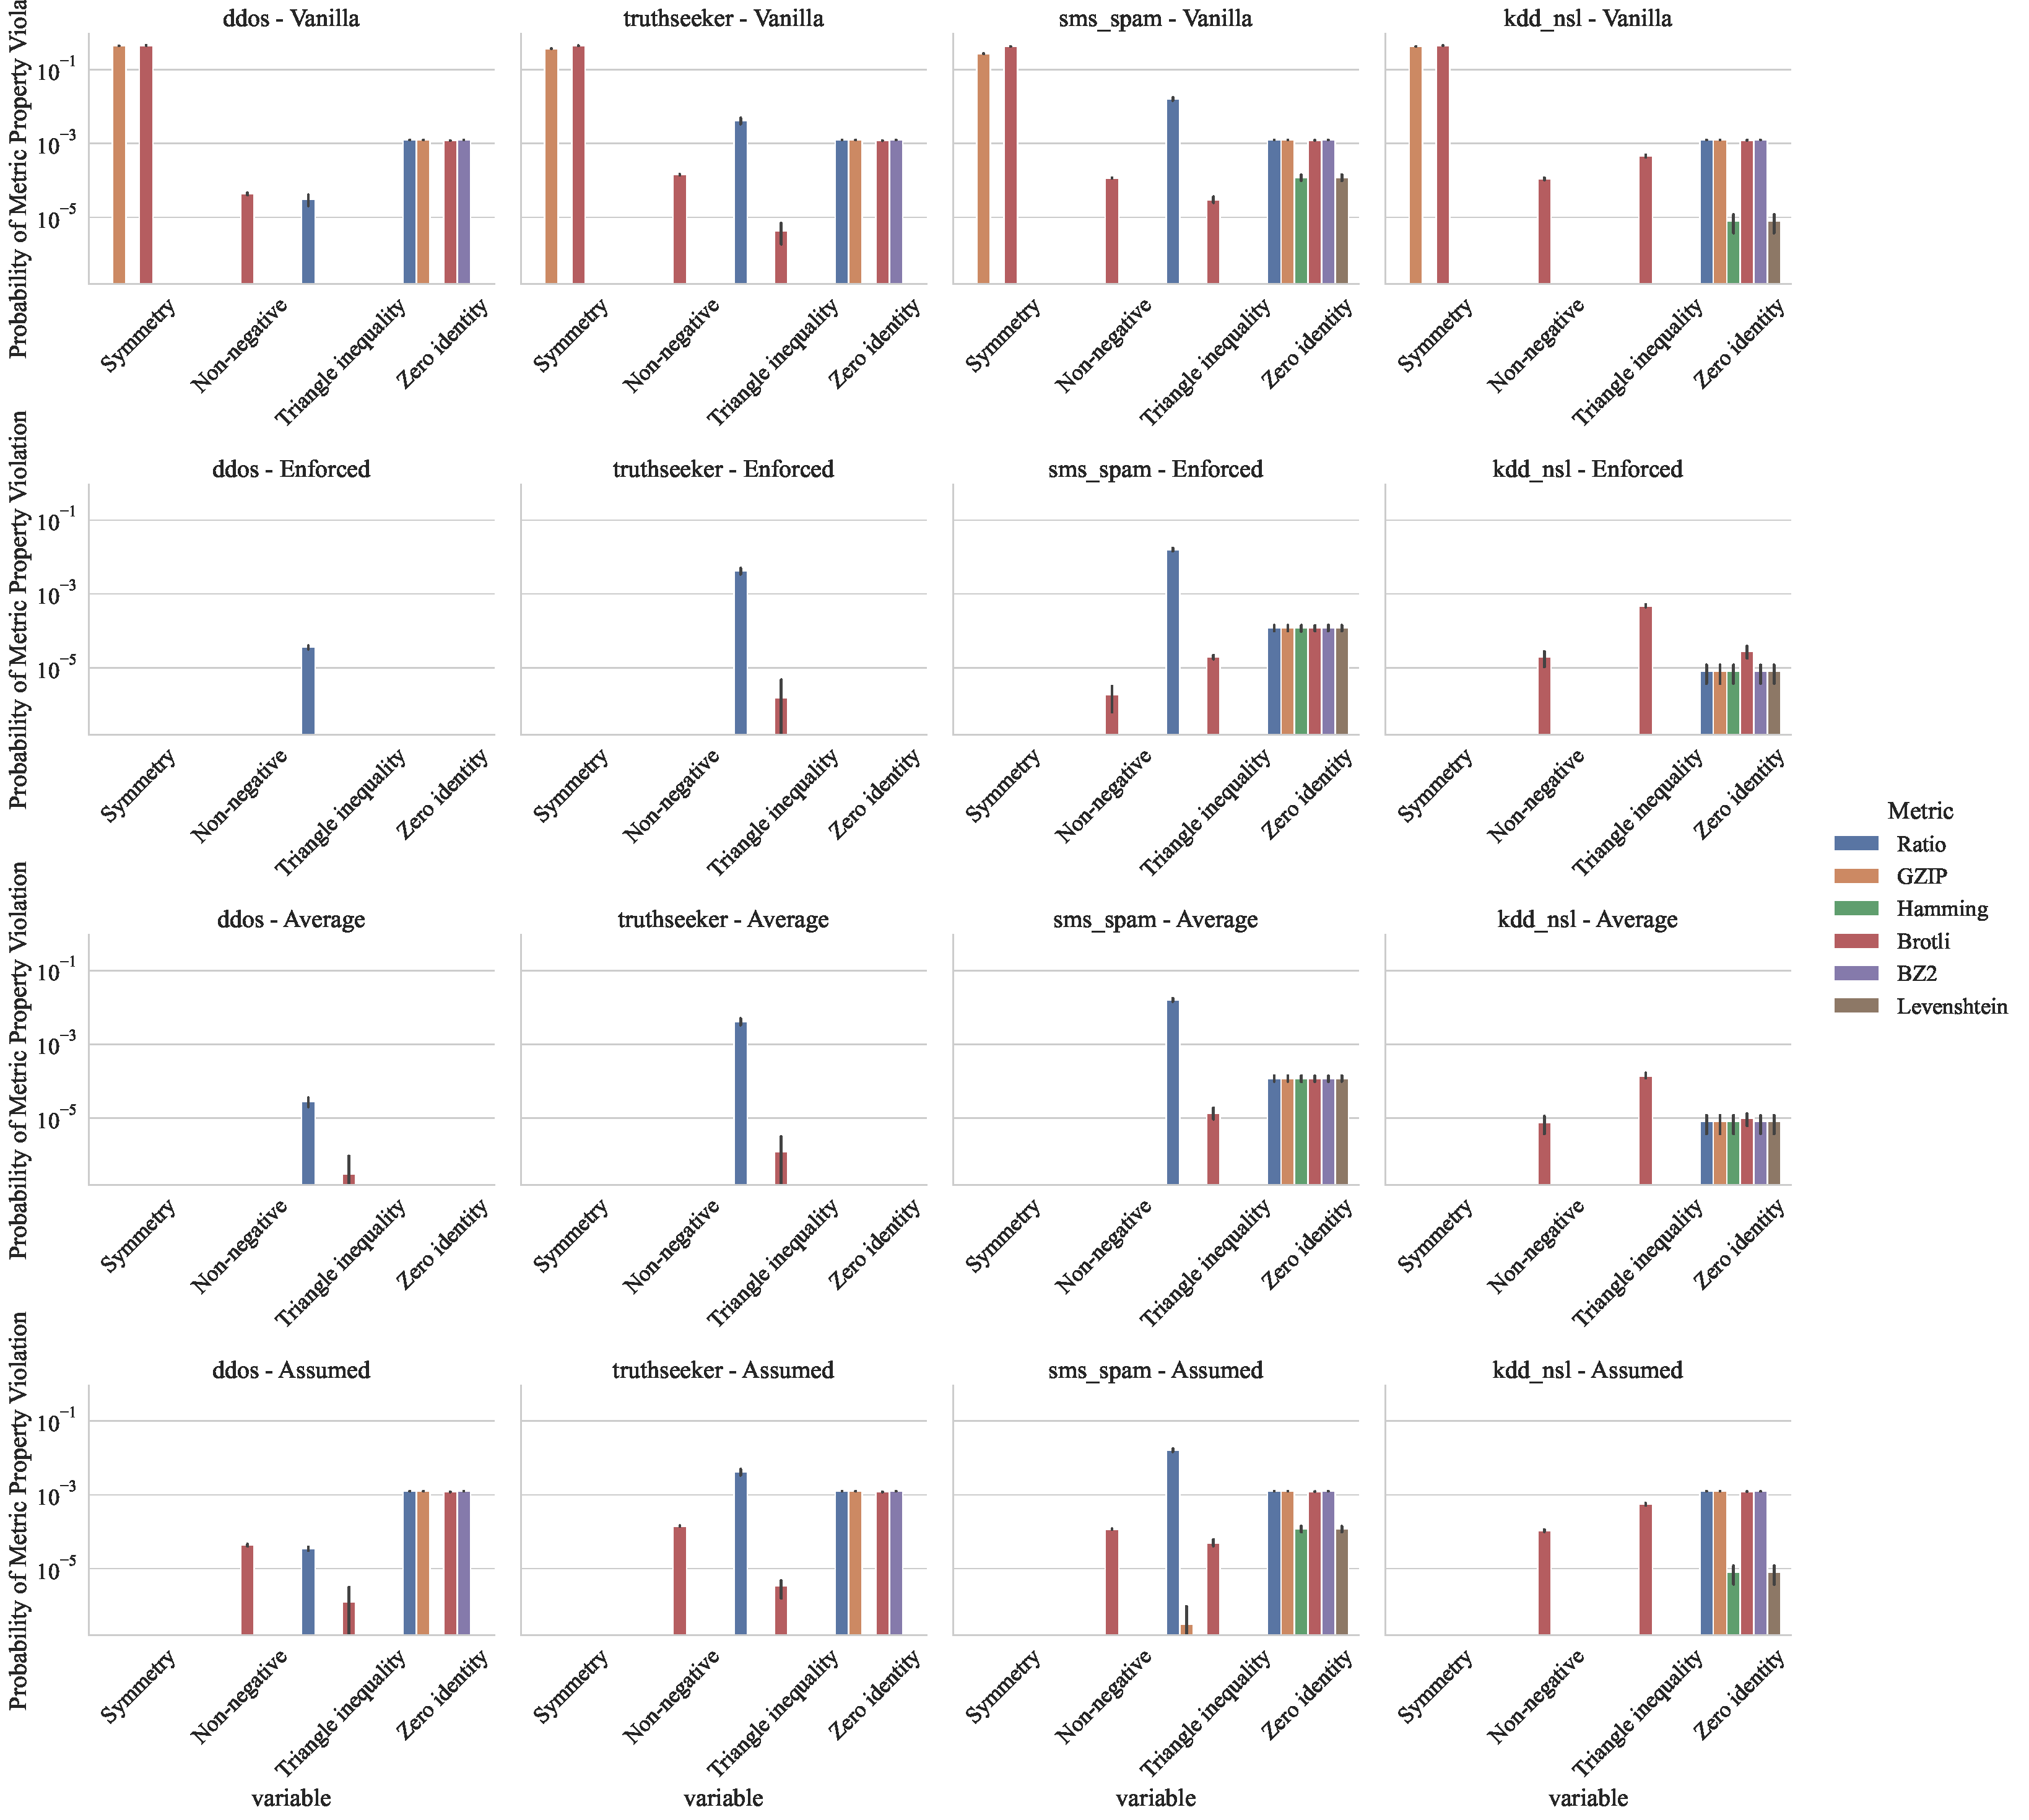
\includegraphics[width=0.99\textwidth]{old_images/read_world_check.pdf}
    \caption{Percentage of examples found that violate the assumptions outlined in Section~\ref{metric_spaces} using the vanilla (Algorithm~\ref{alg:vanilla}, top row), assumed symmetry (Algorithm~\ref{alg:symmetric}, second row), enforced (Algorithm~\ref{eq:assumed}), and averaged (Equation~\ref{eq:average}) algorithms on the training matrices for each of the outlined datasets. Each column is dedicated to a dataset and each model is given a column. The first axis displays which of the axioms is violated and the colour indicates which distance matrix algorithm was used. Since evaluating all possible distance 3-tuples would be computationally infeasible for even hundreds of samples, three disjoint distances were sampled  100 thousand times. \cm{Note: I have fixed the capitalisation in this plot, but am waiting on the new results after changing the ratio metric before re-rendering.}}
    \label{fig:real_world_check}
\end{figure}

Figures~\ref{fig:symmetric_acc}~and~\ref{fig:kernel_acc} depict the accuracy (top), Figure~\ref{fig:distance_time} depicts the training time per sample, and Figure~\ref{fig:pred_time} depicts the inference time per sample (bottom) for each algorithm (denoted by colour and outlined in Section~\ref{modifications}).
The accuracy of the various symmetricisation algorithm varies significantly with dataset, model, and metric and should be treated as a hyper-parameter (Figure~\ref{fig:symmetric_acc}). 
However, the ``Assumed'' and ``Enforced'' versions of the distances are clearly much faster per sample when constructing the distance matrix (Figure~\ref{fig:distance_time}), by reducing the number of distance computations by a factor of around two when compared to the ``Vanilla'' algorithm, which comes at the marginal cost of a few hundred milliseconds for each prediction (Figure~\ref{fig:pred_time}). 
However, the ``Averaged'' algorithm is significantly slower---increasing the distance matrix calculation time by roughly two times over the ``Vanilla'' method.
Overall, it is clear that these symmetricisation algorithms offer improvements in accuracy (Figure~\ref{fig:symmetric_acc}), run-time (Figure~\ref{fig:distance_time}) or both when compared to the ``Vanilla'' distance matrix computation algorithm.



\subsection{Run-time Considerations}

Figure~\ref{fig:distance_time} depicts the time needed to compute the distance matrix per sample in the training set for each dataset (column), algorithm (colour), and metric (first axis).
It is clear that the run-times of the string distance metrics (Figure~\ref{fig:distance_time}) are fairly consistent across the datasets and that the proposed run-time improvements (denoted ``Assumed'' and ``Enforced'') do decrease the distance matrix calculation time with no resulting loss in accuracy (see Figure~\ref{fig:symmetric_acc}).
While the symmetric extension of NCD (denoted ``Averaged'') does take significantly more time than the other distance matrix algorithms ((Figure~\ref{fig:distance_time}), that marginal increase is mere milliseconds in practice and is guaranteed to be symmetric without assuming or enforcing symmetry ((Figure~\ref{fig:distance_time}).
However, Hamming distance takes substantially more time than other metrics on the DDoS dataset and GZIP takes substantially more time than the other metrics on the KDD NSL dataset.
This exceptional run-time can be mitigated by considering the run-time costs during the model training stage since these string distance metrics take longer but do not result in substantially better accuracies for those datasets (see Figure~\ref{fig:metric_acc}).

Figure~\ref{fig:train_time} depicts the time needed to train a model on one pairwise distance calculation, averaged across all experiments, where it is clear that even when the prediction times vary between symmetricisation algorithm, that the marginal cost is no more than a millisecond with total times no larger than 3 milliseconds per sample.
Figure~\ref{fig:pred_time} depicts the time needed to predict a new classification on a single sample for each dataset (column), symmetricisation algorithm (colour) and metric (first axis).
The prediction time per sample (after calculating the distance between a new sample and those in the training set) is 10s of milliseconds across all distances, datasets, models, and metrics, though the branching logic introduced by the ``Assumed'' and ``Enforced'' algorithms does increase the model latency by a fraction of a millisecond (Figure~\ref{fig:pred_time}).
Overall, it is clear that the proposed symmetricisation algorithms are effective (Figures~\ref{fig:distance_time}~and~\ref{fig:symmetric_acc}) and that NCD can be plausibly used in real-time, client-side settings.
It is clear that the time needed to do the compression (Figure~\ref{fig:distance_time}) is a larger factor in the resulting run-time than either the model training (Figure~\ref{fig:train_time}) or model prediction (Figure~\ref{fig:pred_time}), though models with many hyper-parameters would need to be tuned for each user and this run-time can be significant.


\begin{figure}[H]
    \centering
    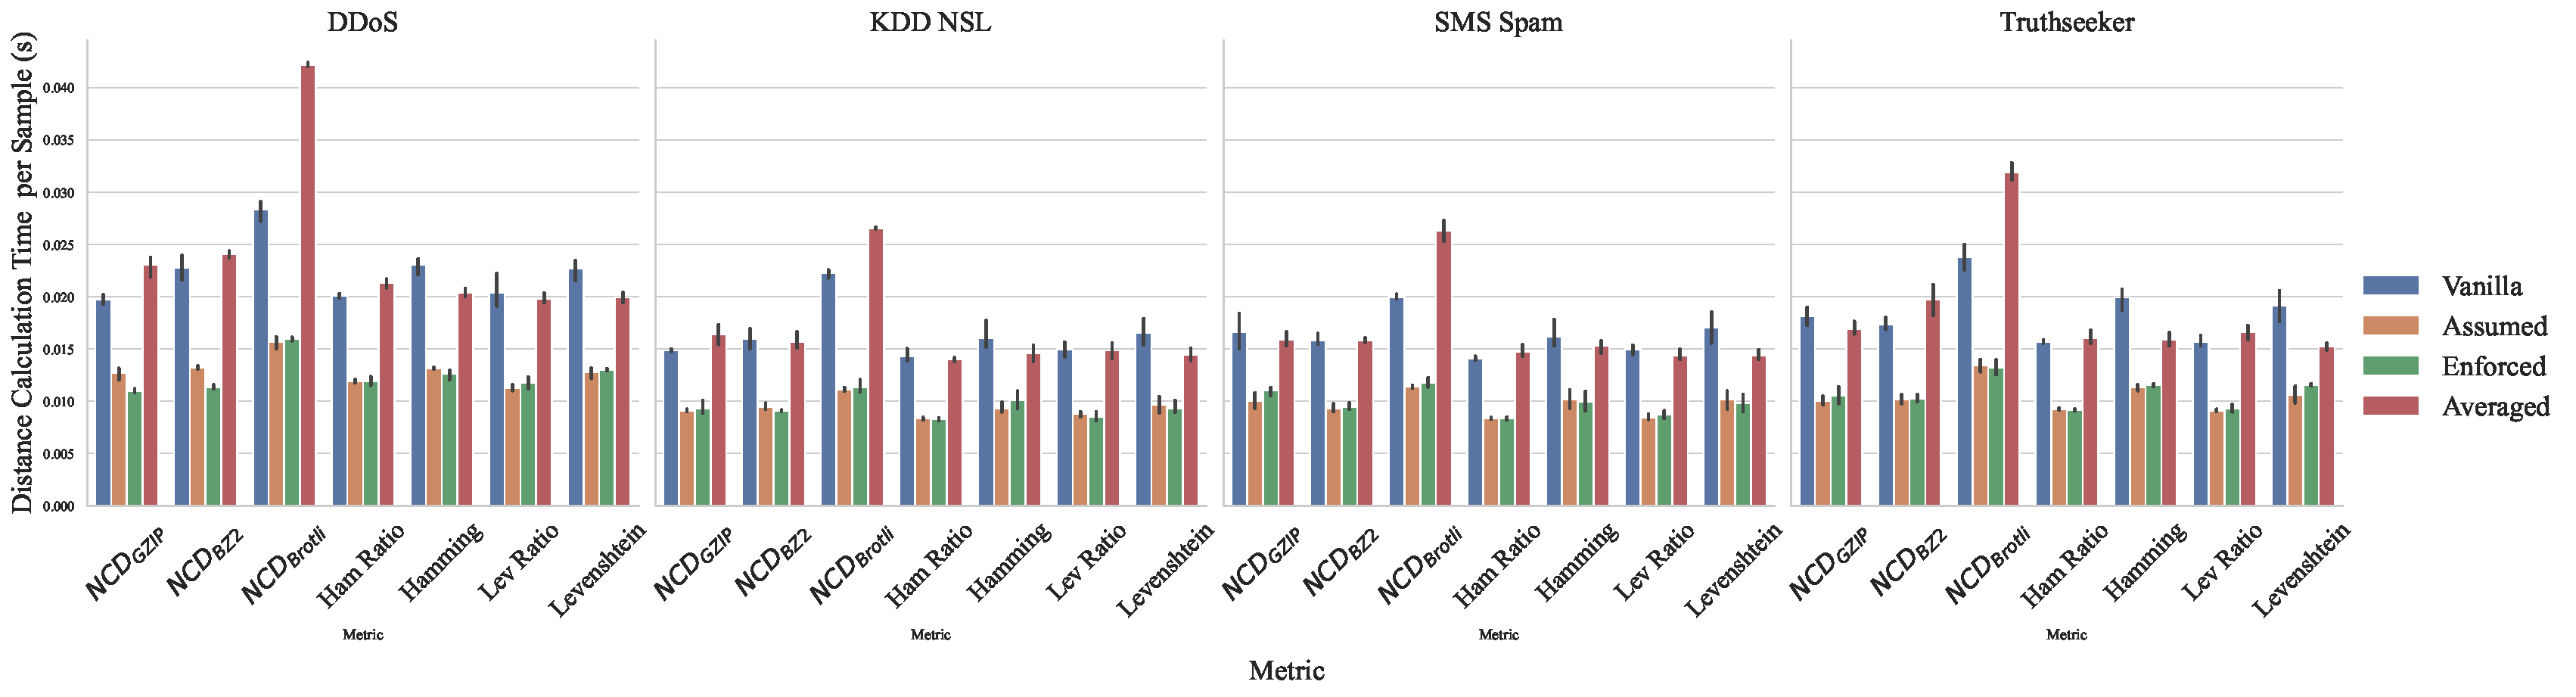
\includegraphics[width=0.99\textwidth]{images/distance_time_vs_symmetry.pdf}
    \caption{The distance matrix calculation time per sample for each metric (first axis), dataset (columns), and algorithm (colour). Because the distance matrix was only calculated once per dataset/algorithm/metric combination there is no differentiation between the models.}
    \label{fig:distance_time}
\end{figure}

\begin{figure}[H]
    \centering
    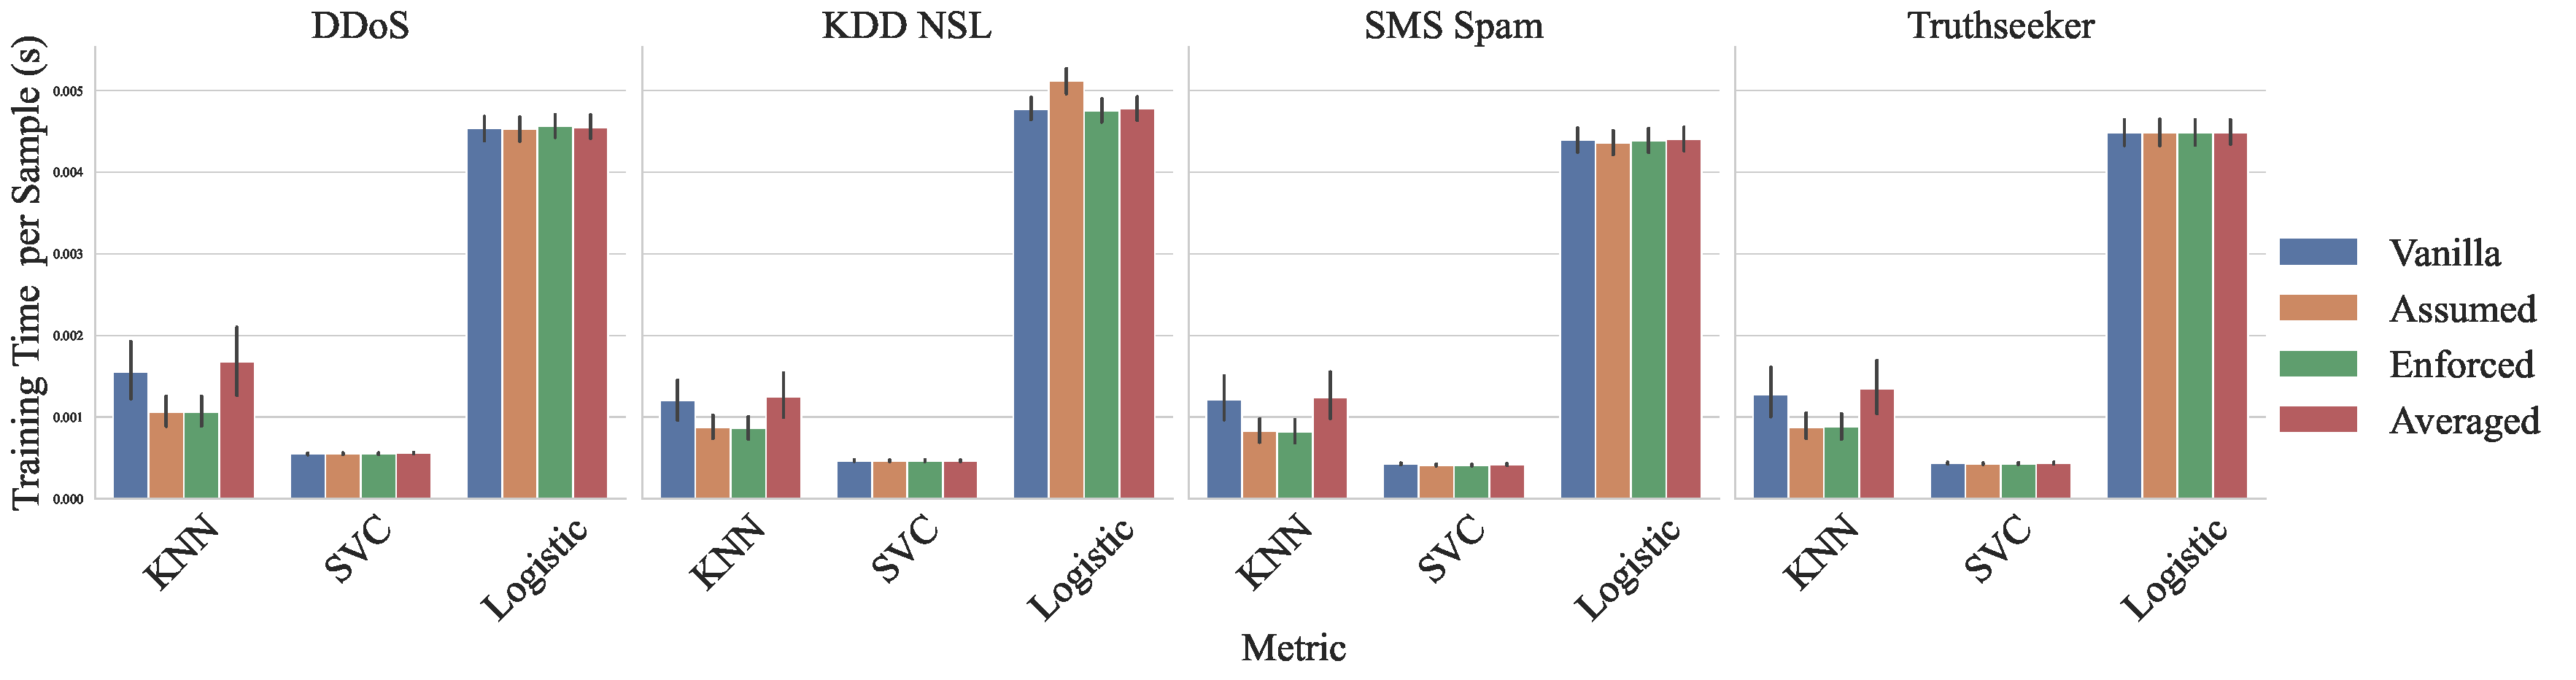
\includegraphics[width=0.99\textwidth]{images/train_time_vs_symmetry.pdf}
    \caption{The training time  per sample (after computing the distance matrix) for each metric (first axis), dataset (rows), model (columns) and algorithm (colour).}
    \label{fig:train_time}
\end{figure}

\begin{figure}[H]
    \centering
    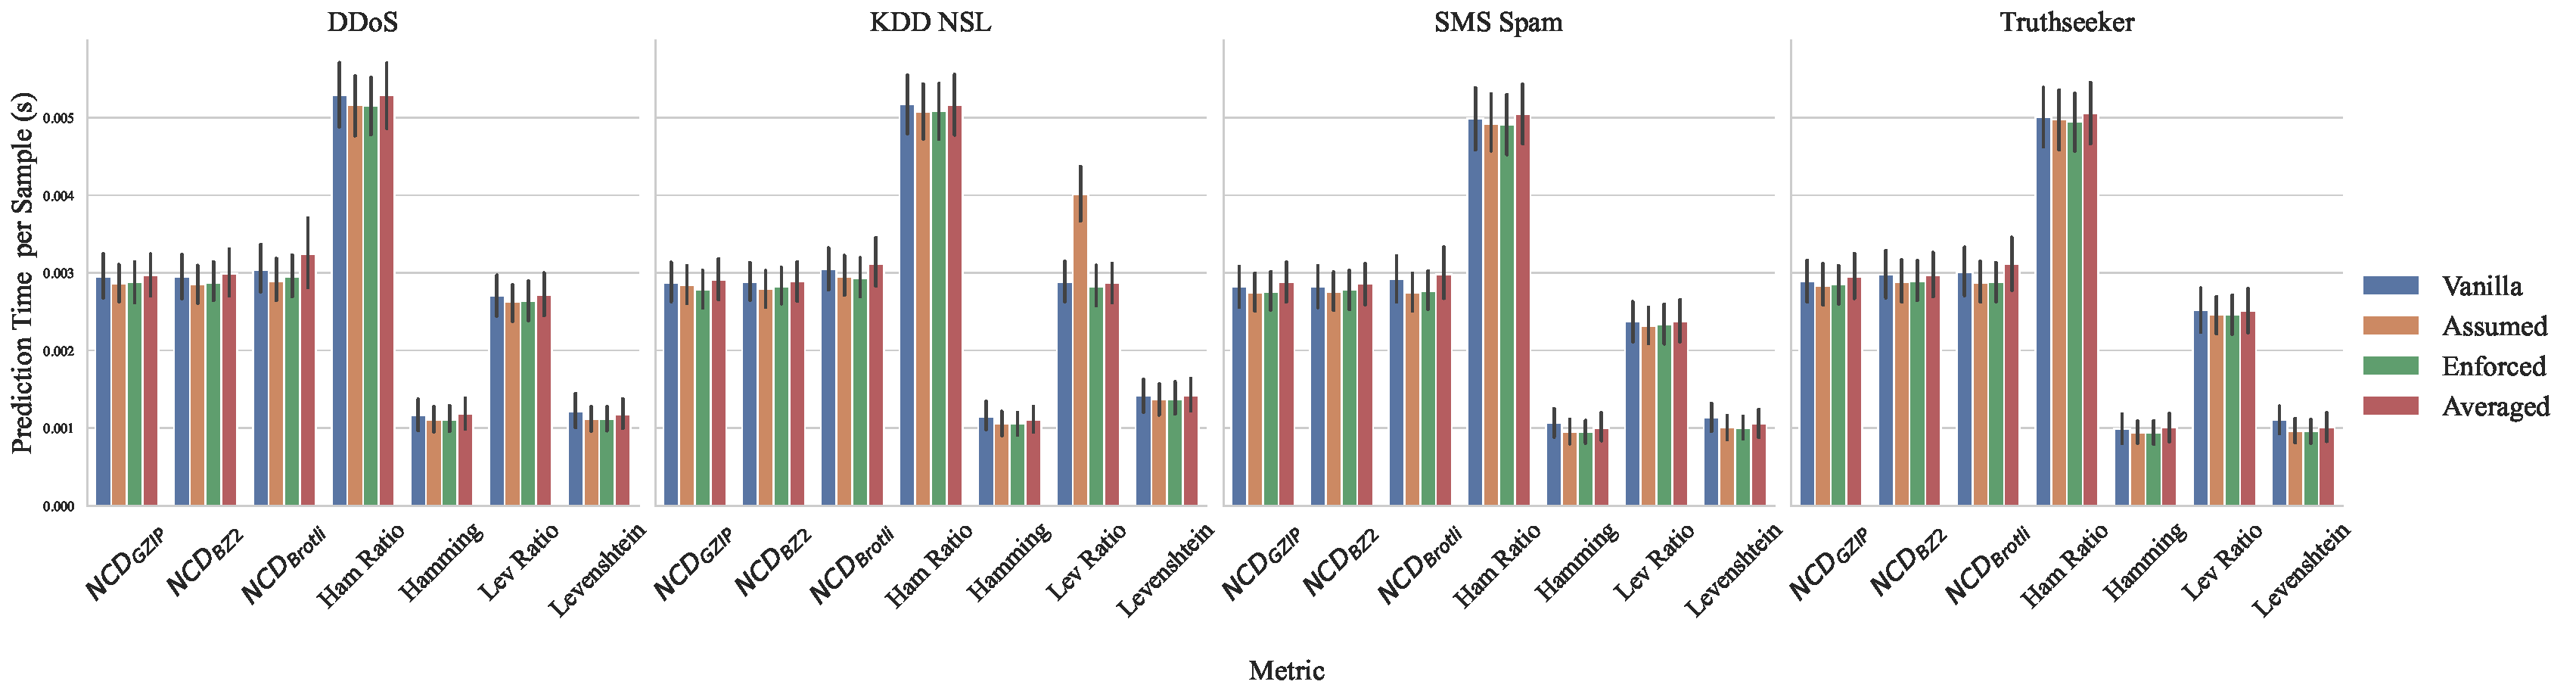
\includegraphics[width=0.99\textwidth]{images/pred_time_vs_symmetry.pdf}
    \caption{The predictions time per sample (after computing the distance matrix) for each metric (first axis), dataset (rows), model (columns) and algorithm (colour).}
    \label{fig:pred_time}
\end{figure}



\subsection{Sample Size Considerations}
\begin{figure}[h]
    \centering
    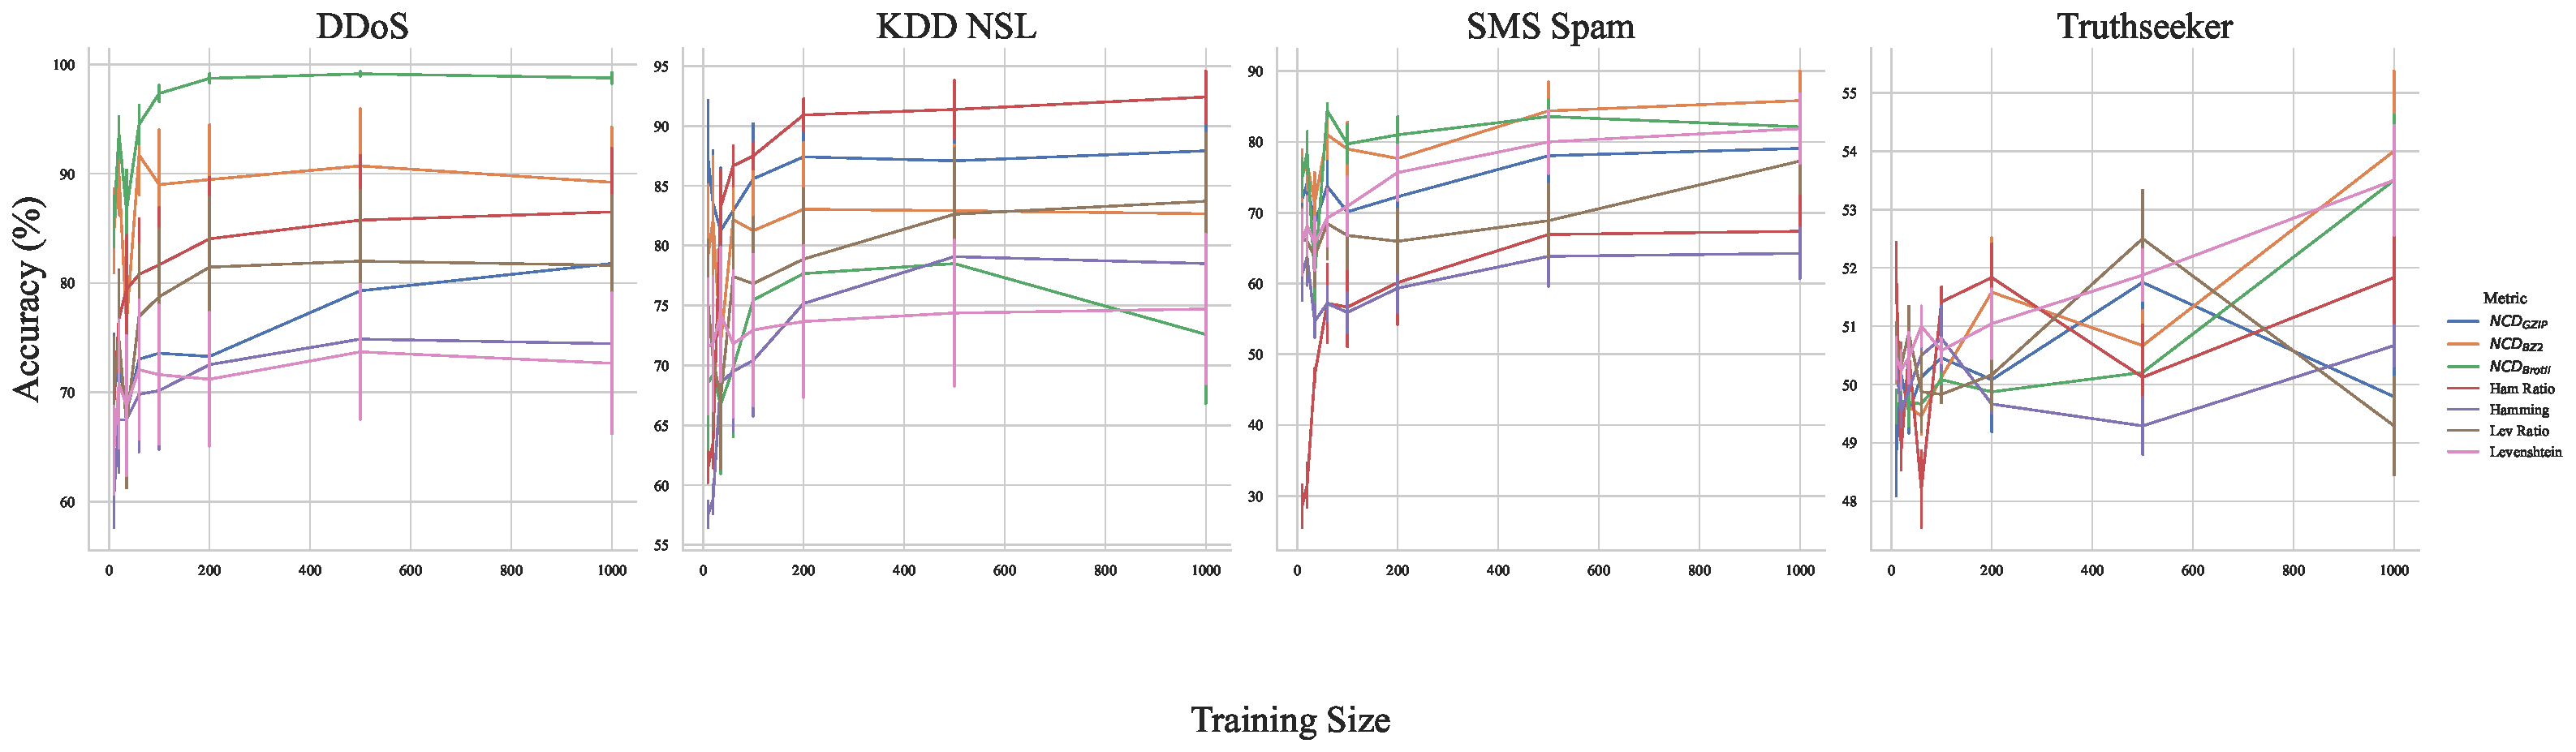
\includegraphics[width=0.99\textwidth]{images/accuracy_vs_sample_size_vs_metric.pdf}
    \caption{The accuracy for each metric (colour), dataset (column) across all models and symmetricisation algorithms as the number of training samples varies (first axis) computed on 200 samples that were withheld in the cross-validation (as reported in Figures~\ref{fig:metric_acc} and~\ref{fig:symmetric_acc}).}
    \label{fig:sample_size}
\end{figure}

\begin{figure}[h]
    \centering
    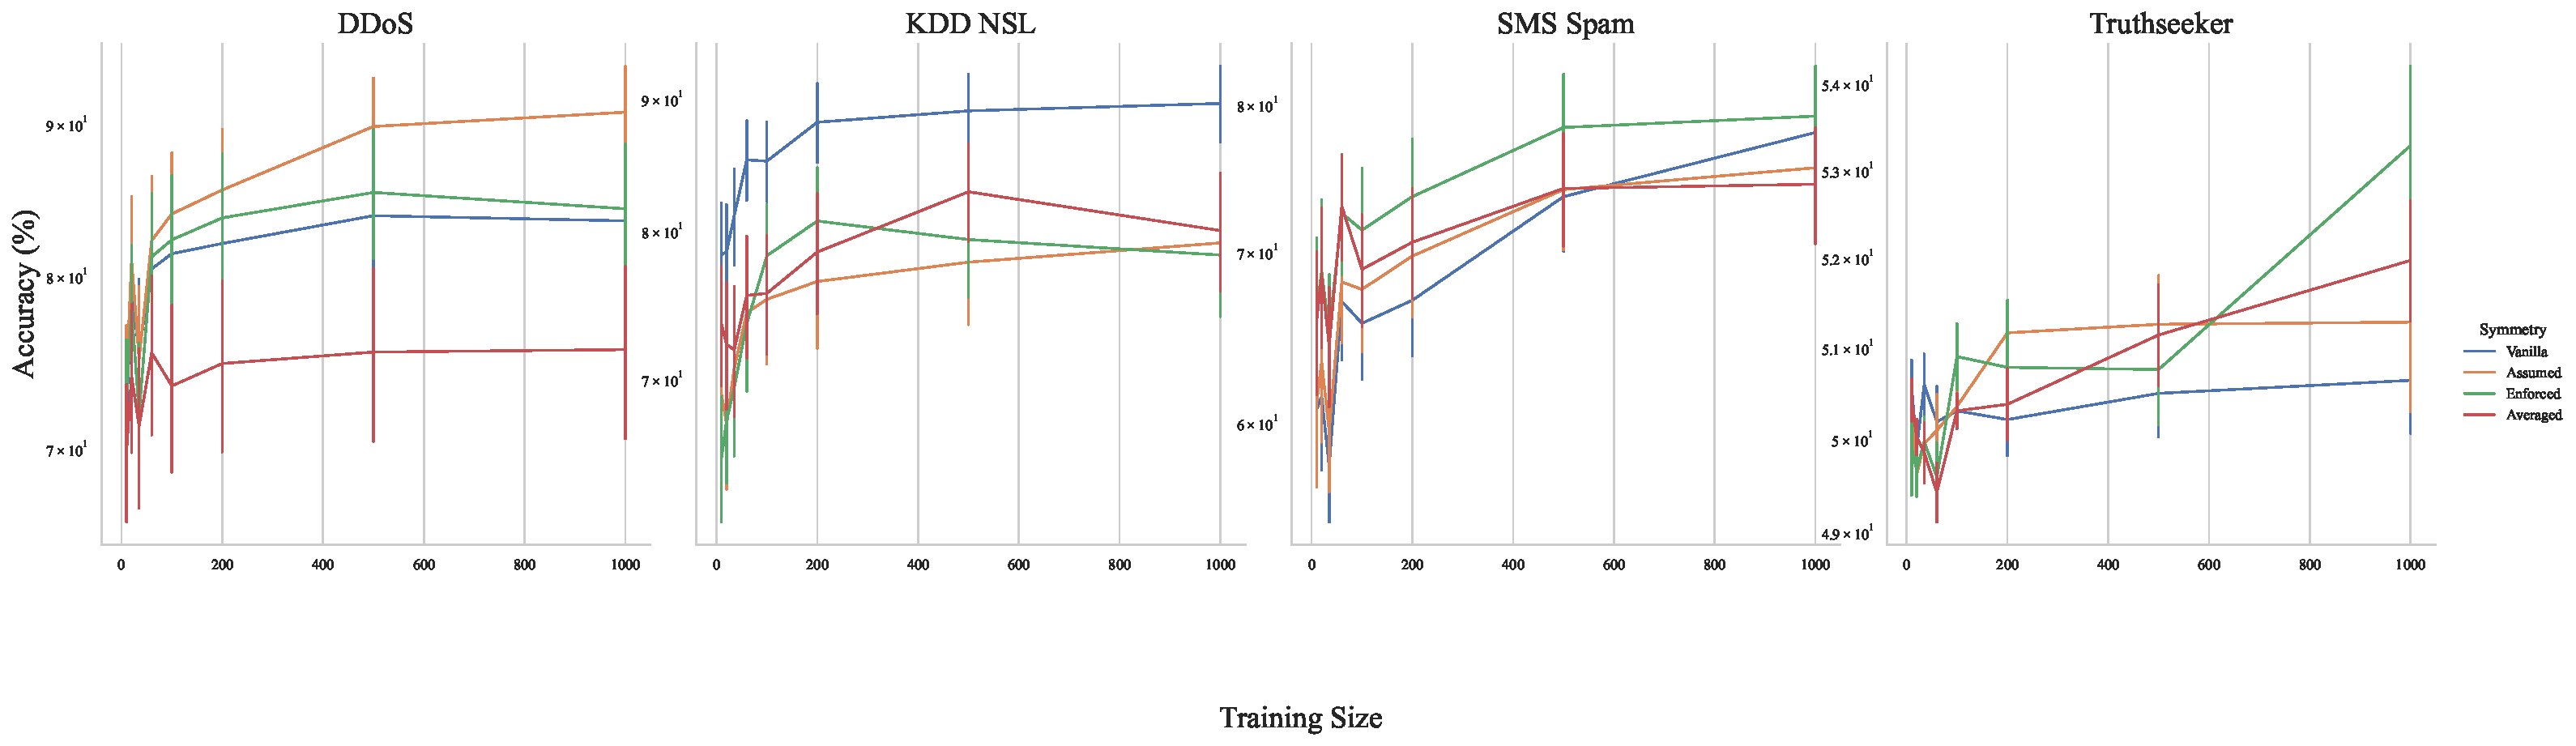
\includegraphics[width=0.99\textwidth]{images/accuracy_vs_sample_size_vs_symmetric.pdf}
    \caption{The accuracy for each symmetricisation algorithm (colour), dataset (column) across all models and metrics as the number of training samples varies (first axis) computed on 200 samples that were withheld in the cross-validation (as reported in Figures~\ref{fig:metric_acc} and~\ref{fig:symmetric_acc}).}
    \label{fig:sample_size_symmetric}
\end{figure}

Figure~\ref{fig:sample_size} depicts the accuracy of the best-performing model for each dataset (column), metric (colour) for a number of different sample sizes (first axis) using 200 left-out validation samples from the cross-validation.
Figure~\ref{fig:sample_size_symmetric} depicts the accuracy of the best-performing model for each dataset (column) and symmetricisation algorithm (colour) for a number of different sample sizes (first axis) using 200 left-out validation samples from the cross-validation.

It is clear that NCD is quite effective even on tens of samples and that the accuracy tends to converge quickly across datasets, models, metrics, and distance matrix algorithms.
It is also clear that NCD tends to outperform other string metrics when the number of samples is small (see Figure~\ref{fig:sample_size}) and that the symmetricisation algorithms can outperform the vanilla distance computation algorithm, though this result is not consistent (see Figure~\ref{fig:sample_size_symmetric}). 
As such, the symmetricisation algorithm should be treated as a tunable hyper-parameter.







\section{Limitations}
\label{limitations}

Since one goal of this work was to produce an algorithm that focuses on user-privacy rather than absolute accuracy, it is necessary to discuss the limitations of this client-side approach to classification.
For example, even if a model is trained entirely on private data and stored privately, the model itself can still be targeted by cross-site scripting attacks~\cite{}, though these can be prevented categorically using best practices~\cite{}. 
However, due to the remarkable efficacy of NCD when used as a kernel method on even a small number of samples (Figure~\ref{fig:sample_size}) and run-times on the order of a few milliseconds (Figures~\ref{fig:distance_time}-\ref{fig:pred_time}), the proposed string metric can be used to train and deploy models entirely on a client device, thus reducing the attack surface to user-error (\textit{e.g.} sharing the trained model through a third-party application) or the aforementioned cross-site scripting attacks. 
Nevertheless, automated spam detection systems raise broad censorship and surveillance concerns~\cite{chat_control} that are not solved here. 
However, the hope of the authors is that distributed and diverse models, trained on data from individual users rather than centrally deployed spam filters reduce the risks of censorship associated with models and data controlled by private interests~\cite{chat_control}. 
To further improve the run-time, compression algorithms designed specifically to exploit graphics processing units have been developed and large datasets would be likely to benefit from these implementations over the CPU-based implementations presented in this paper~\cite{compression_gpu}. 





\section{Conclusion}
\label{conclusion}

Overall, we see that NCD is at least as accurate as other string metrics (Figure~\ref{fig:metric_acc}), despite not being a true metric (Section~\ref{pseudometric}). 
Furthermore, we see that the proposed symmetricisation algorithms are quite effective--sometimes even outperforming the ``Vanilla'' method (Figure~\ref{fig:symmetric_acc}). 
It is clear from Figures~\ref{fig:metric_acc}--\ref{fig:pred_time} that the ``Assumed'' and ``Enforced'' symmetricisation algorithms proposed in this work are superior to those found in the literature by decreasing the run-time without penalising accuracy.
In some cases, the ``Averaged'' symmetricisation algorithm offers superior accuracy over the other methods (Figure~\ref{fig:symmetric_acc}) while inducing a marginal cost of only a few milliseconds (Figure~\ref{fig:distance_time}).
By reducing the chance of erroneous zero distances and enforcing symmetry, the proposed modifications induce metricity that can improve the accuracy of kernel-based classification models (Figure~\ref{fig:symmetric_acc}).
NCD can reach more than 95\% accuracy on even tens of samples (Figure~\ref{fig:sample_size}).
The proposed model is a real-time, client-side classification algorithm that can be trained on a very small number of samples--potentially collected from only a single user.
By training a model for each user, session, and/or device, model database poisoning attacks~\cite{biggio_poisoning_2013} are categorically avoided.
Furthermore, the proposed model reduces the attack surface of attacks like model inference attacks, database exfiltration attacks, and evasion attacks since a malicious user would need to target the personalised classifier of each user session, and/or device~\cite{biggio_evasion_2013,deepfool,chakraborty_adversarial_2018,extraction_attack}.
While it is known that some attacks are quite transferable~\cite{wang2021enhancing}, the proposed model reduces the common attack surface to \textit{only} samples that are universal for all users. 
The end result is a model with a substantially reduced attack surface that is nevertheless accurate.



\bibliographystyle{elsarticle-num} 
\bibliography{bibliography}

\end{document}
